% % % % % % % % % % % % % % % % % % % % % % % % % % % % % % % % % % % % % % % %
% LaTeX4EI Template for Cheat Sheets                                Version 1.0
%
% Authors: Emanuel Regnath, Martin Zellner
% Contact: info@latex4ei.de
% Encode: UTF-8, tabwidth = 4, newline = LF
% % % % % % % % % % % % % % % % % % % % % % % % % % % % % % % % % % % % % % % %


% ======================================================================
% Document Settings
% ======================================================================

% possible options: color/nocolor, english/german, threecolumn
% defaults: color, english
\documentclass[english]{latex4ei/latex4ei_sheet}

% set document information
\title{Adaptive and Array\\ Signal Processing}
\author{Johannes Kunz}					% optional, delete if unchanged
\myemail{info@latex4ei.de}			% optional, delete if unchanged
\mywebsite{www.latex4ei.de}			% optional, delete if unchanged


\let\T\relax
\DeclareMathOperator{\T}{\textsf{\textit{T}}}		% Zufallsvariable X
\DeclareMathOperator{\Bias}{Bias}		% Zufallsvariable X
\DeclareMathOperator{\argmax}{argmax}

\DeclareMathOperator{\rang}{rang}
\renewcommand{\vec}[1]{\underline{\boldsymbol{#1}}}
%\renewcommand{\vec}[1]{\boldsymbol{#1}}



\newcommand{\x}{\textit{x}}
\newcommand{\vx}{\underline{\textbf{\textit{x}}}}
\newcommand{\VX}{\underline{\textbf{\textit{X}}}}

\newcommand{\y}{\textit{y}}
\newcommand{\vy}{\underline{\textbf{\textit{y}}}}
\newcommand{\VY}{\underline{\textbf{\textit{Y}}}}


\newcommand{\VA}{\underline{\textit{A}}}
\newcommand{\A}{\textit{A}}
\newcommand{\va}{\underline{\textbf{\textit{a}}}}

\newcommand{\VB}{\underline{\textit{B}}}
\newcommand{\danger}[1]{\textcolor{red}{#1}}

\newcommand{\comment}[1]{\textcolor{red}{#1}}

\newcommand{\vfsymbol}[1][]{\mbox{\setlength{\unitlength}{0.1em}%
                            \begin{picture}(15,18)%
                              \put(6,2){\circle*{4}}%
                              \put(6,4){\line(0,1){12}}%
                              \put(6,18){\circle{4}}%
                              \put(13,7){#1}
                            \end{picture}%
                           }%
                     }%
                     
\newcommand{\fsymbol}[1][]{\mbox{\setlength{\unitlength}{0.1em}%
                            \begin{picture}(30,10)%
                              \put(6,4){\circle{4}}%
                              \put(6,4){\line(1,0){12}}%
                              \put(21,4){\circle*{4}}%
                              \put(14,7){#1}
                            \end{picture}%
                           }%
                     }%
                     
\newcommand{\finvsymbol}[1][]{\mbox{\setlength{\unitlength}{0.1em}%
                            \begin{picture}(30,10)%
                              \put(6,4){\circle*{4}}%
                              \put(6,4){\line(1,0){12}}%
                              \put(21,4){\circle{4}}%
                              \put(14,7){#1}
                            \end{picture}%
                           }%
                     }%

\usepackage{multirow}


% ======================================================================
% Begin
% ======================================================================
\begin{document}

\IfFileExists{git.id}{\input{git.id}}{}
\ifdefined\GitRevision\mydate{\GitNiceDate\ (git \GitRevision)}\fi
% Title
% ----------------------------------------------------------------------
\maketitle   % requires ./img/Logo.pdf


\section{Complex Analysis}
\begin{sectionbox}
\subsection{Derivatives of Non-analytic functions}
\begin{emphbox}
  $h: \mathbb{C} \ni z \mapsto h(z) \in \mathbb{C}$\\
  $f: \mathbb{R}^{2} \ni(x, y) \mapsto f(x, y) \in \mathbb{C}$, $z=x+jy$\\
  $g: \mathbb{C}^{2} \ni\left(z_{1}, z_{2}\right) \mapsto g\left(z_{1}, z_{2}\right) \in \mathbb{C}$, $x=\frac{z+z^{*}}{2}, y=\frac{z-z^{*}}{2 \mathrm{j}}$
\end{emphbox}
Derivative in direction $\varphi$:\\
$\frac{\mathrm{d} h}{\mathrm{~d} z}=\left(\frac{\partial f}{\partial x} \cos (\varphi)+\frac{\partial f}{\partial y} \sin \varphi\right) \mathrm{e}^{-\mathrm{j} \varphi}$, $\mathrm{d} z=\mathrm{e}^{\mathrm{j} \varphi} \mathrm{d} t, \quad \varphi, \mathrm{d} t \in \mathbb{R}$\\
\begin{emphbox}
  $\frac{\partial g}{\partial z}=\frac{1}{2}\left(\frac{\partial f}{\partial x}-\mathrm{j} \frac{\partial f}{\partial y}\right), \quad \frac{\partial g}{\partial z^{*}}=\frac{1}{2}\left(\frac{\partial f}{\partial x}+\mathrm{j} \frac{\partial f}{\partial y}\right)$
\end{emphbox}

\end{sectionbox}


\begin{sectionbox}
\subsection{Analytic functions}
Definition:
\begin{emphbox}
  $\frac{\mathrm{d} h}{\mathrm{~d} z}$ independent of $\varphi$\\
  $\forall(x, y) \in \mathbb{R}^{2}: \quad \frac{\partial f}{\partial x}+j \frac{\partial f}{\partial y}=0$\\
  $\frac{\mathrm{d} h}{\mathrm{~d} z}=\frac{\partial f}{\partial x}=-\mathrm{j} \frac{\partial f}{\partial y}$\\
  $\frac{\partial g}{\partial z^{*}} \equiv 0$
\end{emphbox}
\begin{itemize}
  \item Ansatz for obtaining the Lemma: compute derivative of $\frac{\mathrm{d} h}{\mathrm{~d} z}$ wrt. to $\varphi$ and set it to 0.
  \item If $g()$ depends on $z^*$ it is not analytic
\end{itemize}
\end{sectionbox}

\begin{sectionbox}
  \subsection{Minimization of $h(z)=g\left(z, z^{\star}\right) \in \mathbb{R}$}
  \begin{emphbox}
    Necessary condition for an extremum:\\
    $\frac{\partial g}{\partial z^{\star}}=0$
  \end{emphbox}
  Direction of steepest descent: $z \leftarrow z-\mu \frac{\partial g}{\partial z^{\star}}, \quad \mu>0$\\
  \begin{emphbox}
    Useful derivatives:\\
    $\frac{\partial\left(\boldsymbol{z}^{\mathrm{H}} \boldsymbol{p}+\boldsymbol{p}^{\mathrm{H}} \boldsymbol{z}\right)}{\partial \boldsymbol{z}^{\star}} = \boldsymbol{p}$\\
    $\frac{\partial\left(\boldsymbol{z}^{\mathrm{H}} \boldsymbol{R} z\right)}{\partial \boldsymbol{z}^{*}}=\boldsymbol{R}\boldsymbol{z}$\\
    $\frac{\partial \operatorname{tr}\left(\boldsymbol{S}^{\mathrm{H}} \boldsymbol{B}\right)}{\partial \boldsymbol{S}^{*}} = \boldsymbol{B}$
  \end{emphbox}
\end{sectionbox}

\begin{sectionbox}
  \subsection{Quadratic minimization with linear equality constraints}
  \textbf{Problem:}\\
  $\min _{\boldsymbol{z}} \boldsymbol{z}^{\mathrm{H}} \boldsymbol{R} \boldsymbol{z}, \quad \text { such that } \quad \boldsymbol{A}^{\mathrm{H}} \boldsymbol{z}=\boldsymbol{b}, \quad \boldsymbol{R}=\boldsymbol{R}^{\mathrm{H}}>\boldsymbol{0}$\\
  
  \textbf{Corresponding Lagrange-ian function:}\\
  $\mathcal{L}=\boldsymbol{z}^{\mathrm{H}} \boldsymbol{R} \boldsymbol{z}+\boldsymbol{\lambda}^{\mathrm{H}}\left(\boldsymbol{A}^{\mathrm{H}} \boldsymbol{z}-\boldsymbol{b}\right)+\left(\boldsymbol{z}^{\mathrm{H}} \boldsymbol{A}-\boldsymbol{b}^{\mathrm{H}}\right) \boldsymbol{\lambda}$\\

  \textbf{Resulting dual optimization problem:} $\min _{z} \max _{\lambda} \mathcal{L}$\\

  \textbf{Solution:}
  \begin{emphbox}
    \vspace{-0.2cm}
    $$\boldsymbol{z}_{\mathrm{opt}}=\boldsymbol{R}^{-1} \boldsymbol{A}\left(\boldsymbol{A}^{\mathrm{H}} \boldsymbol{R}^{-1} \boldsymbol{A}\right)^{-1} \boldsymbol{b}$$
    $$\operatorname{min} \boldsymbol{z}^H\boldsymbol{R}\boldsymbol{z} = \boldsymbol{b}^H(\boldsymbol{A}^H\boldsymbol{R}^{-1}\boldsymbol{A})^{-1}\boldsymbol{b}$$
  \end{emphbox}

\end{sectionbox}

\begin{sectionbox}
  \subsection{Real-valued quadratic minimization with linear inequality constraints}
  \textbf{Problem:}\\
  $\min _{\boldsymbol{x}} \boldsymbol{x}^{\mathrm{T}} \boldsymbol{C} \boldsymbol{x}, \quad \text { subject to } \quad \boldsymbol{A} \boldsymbol{x} \leq \boldsymbol{b}$\\  
  
  \textbf{Corresponding Lagrange-ian function:}\\
  $\mathcal{L}=\boldsymbol{x}^{\mathrm{T}} \boldsymbol{C} \boldsymbol{x}+\boldsymbol{\lambda}^{\mathrm{T}}(\boldsymbol{A} \boldsymbol{x}-\boldsymbol{b})$
  
  \textbf{Resulting dual optimization problem:} $\min \max \mathcal{L} \text { subject to } \lambda \geq 0$\\

  \textbf{Algorithm for determining the solution:}
  \begin{center}
    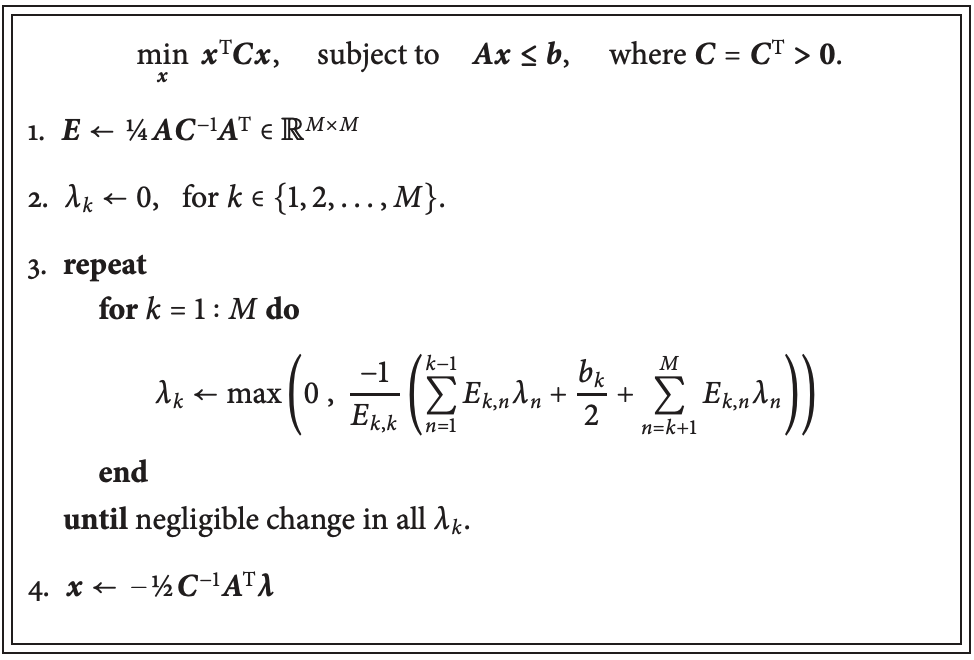
\includegraphics[width = 6.8cm]{img/quadr-opt.png}
  \end{center}
\end{sectionbox}

\section{Linear Algebra}
\begin{sectionbox}
  \subsection{Vector Space}
  A complex vector space $\mathcal{V}$ is a set with the following properties:
  \begin{enumerate}
    \item $\forall \boldsymbol{a}, \boldsymbol{b} \in \mathcal{V}: \quad \boldsymbol{a}+\boldsymbol{b} \in \mathcal{V}$
    \item $\forall \boldsymbol{a}, \boldsymbol{b} \in \mathcal{V}: \quad \boldsymbol{a}+\boldsymbol{b}=\boldsymbol{b}+\boldsymbol{a}$
    \item $\forall \boldsymbol{a}, \boldsymbol{b}, \boldsymbol{c} \in \mathcal{V}: \quad(\boldsymbol{a}+\boldsymbol{b})+\boldsymbol{c}=\boldsymbol{a}+(\boldsymbol{b}+\boldsymbol{c})$
    \item $\forall \boldsymbol{a} \in \mathcal{V}: \exists \mathbf{0} \in \mathcal{V}: \quad \boldsymbol{a}+\mathbf{0}=\boldsymbol{a}$
    \item $\forall \boldsymbol{a} \in \mathcal{V}: \exists-\boldsymbol{a} \in \mathcal{V}: \quad \boldsymbol{a}+(-\boldsymbol{a})=\mathbf{0}$
    \item $\forall \boldsymbol{a} \in \mathcal{V}: \quad 1 \boldsymbol{a}=\boldsymbol{a}$
    \item $\forall \boldsymbol{a} \in \mathcal{V}, \forall \lambda, \mu \in \mathbb{C}: \quad \lambda(\mu \boldsymbol{a})=(\lambda \mu) \boldsymbol{a}$
    \item $\forall \boldsymbol{a}, \boldsymbol{b} \in \mathcal{V}, \forall \lambda \in \mathbb{C}: \quad \lambda(\boldsymbol{a}+\boldsymbol{b})=\lambda \boldsymbol{a}+\lambda \boldsymbol{b}$
    \item $\forall \boldsymbol{a} \in \mathcal{V}, \forall \lambda, \mu \in \mathbb{C}: \quad(\lambda+\mu) \boldsymbol{a}=\lambda \boldsymbol{a}+\mu \boldsymbol{a}$
  \end{enumerate}
\end{sectionbox}

\begin{sectionbox}
  \subsection{Linear Subspace}
  A set $\mathcal{S}$ is called a subspace of a complex vector space $\mathcal{V}$ iff:
  \begin{enumerate}
    \item $\mathcal{S} \subseteq \mathcal{V}$    \item $\forall \boldsymbol{a}, \boldsymbol{b} \in \mathcal{V}: \quad \boldsymbol{a}+\boldsymbol{b}=\boldsymbol{b}+\boldsymbol{a}$
    \item $\forall \boldsymbol{a}, \boldsymbol{b} \in \mathcal{S}: \quad \boldsymbol{a}+\boldsymbol{b} \in \mathcal{S}$
    \item $\forall \boldsymbol{a} \in \mathcal{S}, \forall \lambda \in \mathbb{C}: \quad \lambda \boldsymbol{a} \in \mathcal{S}$
  \end{enumerate}
\end{sectionbox}

\begin{sectionbox}
  \subsection{Linear (In)dependence}
  The vectors $\boldsymbol{v}_{1}, \ldots, \boldsymbol{v}_{n} \in \mathcal{V}$ are said to be linearly independent iff:\\
  $\sum_{k=1}^{n} a_{k} \boldsymbol{v}_{k}=\mathbf{0} \quad \Longrightarrow \quad a_{1}=\cdots=a_{n}=0$\\
  
  The vectors are linearly dependent iff:\\
  $\exists i: \exists b_{1}, \ldots, b_{i-1}, b_{i+1}, \ldots, b_{n} \in \mathbb{C}: \quad \boldsymbol{v}_{i}=\sum\limits_{k=1, k \neq i}^{n} b_{k} \boldsymbol{v}_{k}$\\

  \begin{itemize}
    \item $\boldsymbol{v}_{1}, \ldots, \boldsymbol{v}_{n} \in \mathcal{V} \text { are } L I, \text { and } \boldsymbol{s} \in \mathcal{V}$ cannot be expressed as a linear combination, then $\boldsymbol{v}_{1}, \ldots, \boldsymbol{v}_{n}, \boldsymbol{s}$ are LI 
    \item $\operatorname{dim}(\mathcal{S})$ of a subspace is the maximum number of LI vectors that fit in it 
    \item For every subspace $\mathcal{S}, \text { with } \operatorname{dim}(\mathcal{S})=n$, and any LI vectors $\boldsymbol{v}_{1}, \ldots, \boldsymbol{v}_{n} \in \mathcal{S}$ we have $\mathcal{S}=\operatorname{Sp}\left(\boldsymbol{v}_{1}, \ldots, \boldsymbol{v}_{n}\right)$ 
    \item Orthonormal vectors are LI 
  \end{itemize}
\end{sectionbox}

\begin{sectionbox}
  \subsection{Gram-Schmidt}
  $\boldsymbol{u}_{2}=\boldsymbol{v}_{2}-\boldsymbol{u}_{1} \frac{\boldsymbol{u}_{1}^{\mathrm{H}} \boldsymbol{v}_{2}}{\boldsymbol{u}_{1}^{\mathrm{H}} \boldsymbol{u}_{1}} \dots$\\
\end{sectionbox}

\begin{sectionbox}
  \subsection{Matrix Cookbook}
  $\operatorname{tr}(\boldsymbol{A} \boldsymbol{B})=\operatorname{tr}(\boldsymbol{B} \boldsymbol{A})$\\
  $\operatorname{tr}(\boldsymbol{CDE})=\operatorname{tr}(\boldsymbol{ECD})=\operatorname{tr}(\boldsymbol{DEC})$\\
  $(\boldsymbol{A} \boldsymbol{B})^{\mathrm{T}}=\boldsymbol{B}^{\mathrm{T}} \boldsymbol{A}^{\mathrm{T}}$\\
  $(\boldsymbol{A B})^{\mathrm{H}}=\boldsymbol{B}^{\mathrm{H}} \boldsymbol{A}^{\mathrm{H}}$\\
  $(\boldsymbol{A} \boldsymbol{B})^{-1}=\boldsymbol{B}^{-1} \boldsymbol{A}^{-1}$\\
  $\left(\boldsymbol{A}^{-1}\right)^{\mathrm{H}}=\left(\boldsymbol{A}^{\mathrm{H}}\right)^{-1}$\\

\end{sectionbox}

\begin{sectionbox}
  \subsection{Determinant}
  $det: \mathbb{C}^{m \times m} \ni \boldsymbol{A} \mapsto \operatorname{det} \boldsymbol{A} \in \mathbb{C}$ having the following properties:
  \begin{enumerate}
    \item $\operatorname{det} \mathbf{I}_{m}=1$
    \item If $\boldsymbol{A}$ has LD columns, then $\operatorname{det} \boldsymbol{A}=0$.
    \item $\operatorname{det} \boldsymbol{A}$ is linear in the columns of $\boldsymbol{A}$.
  \end{enumerate}


  For the determinant of MxM matrices the following is true:
  \begin{enumerate}
    \item For $m=1: \operatorname{det} A=A$.
    \item $\operatorname{det} \boldsymbol{A}=\sum_{i=1}^{m}(-1)^{i+j} A_{i, j} \operatorname{det} \boldsymbol{A}^{[i, j]}$, for any $j \in\{1, \ldots m\}$, where $\boldsymbol{A}^{[i, j]}$ is the matrix that results from $\boldsymbol{A}$ if the $i$-th row and the $j$-th column are removed.
    \item $\operatorname{det}(\boldsymbol{A} \boldsymbol{B})=(\operatorname{det} \boldsymbol{A})(\operatorname{det} \boldsymbol{B})$
    \item $\operatorname{det}\left(\boldsymbol{A}^{-1}\right)=(\operatorname{det} \boldsymbol{A})^{-1}$
    \item $\operatorname{det}\left(\boldsymbol{A}^{\mathrm{T}}\right)=\operatorname{det} \boldsymbol{A}$
  \end{enumerate}
\end{sectionbox}

\begin{sectionbox}
  \subsection{Eigenvalue Decomposition (EVD)}
  \begin{emphbox}
    $\boldsymbol{A}=\boldsymbol{B} \boldsymbol{\Lambda} \boldsymbol{B}^{-1}$
  \end{emphbox}
  $\operatorname{tr} \boldsymbol{A}=\sum_{i=1}^{m} \lambda_{i}$\\
  $\operatorname{det} \boldsymbol{A}=\prod_{i=1}^{m} \lambda_{i}$\\
  $\boldsymbol{A}^{k}=\boldsymbol{B} \boldsymbol{\Lambda}^{k} \boldsymbol{B}^{-1}$\\
  Every scalar function which has a Taylor series expansion can be generalized to matrices:\\
  $\boldsymbol{h}(\boldsymbol{A})=\boldsymbol{B} \boldsymbol{h}(\boldsymbol{\Lambda}) \boldsymbol{B}^{-1}$\\
\end{sectionbox}

\begin{sectionbox}
  \subsection{Hermitian Matrices}
  \begin{emphbox}
    $\boldsymbol{A}=\boldsymbol{A}^H \in \mathbb{C}^{m\times m}$
  \end{emphbox}
  Properties:
  \begin{itemize}
    \item m orthogonal (LI) eigenvectors $\rightarrow$ EVD exists 
    \item real eigenvalues
    \item EVD has the form $\boldsymbol{A}=\boldsymbol{B} \boldsymbol{\Lambda} \boldsymbol{B}^{\mathrm{H}}$
  \end{itemize}

\end{sectionbox}

\begin{sectionbox}
  \subsection{Gramian Matrices}
  \begin{emphbox}
    $\exists \boldsymbol{C} \in \mathbb{C}^{m \times m}: \quad \boldsymbol{A}=\boldsymbol{C} \boldsymbol{C}^{\mathrm{H}}$
  \end{emphbox}
  Properties:
  \begin{itemize}
    \item Hermitian matrix
    \item non-negative real eigenvalues
    \item EVD exists
  \end{itemize}
\end{sectionbox}

\begin{sectionbox}
  \subsection{Sherman-Morrison-Woodbury identity}
  $$(\boldsymbol{A}+\boldsymbol{B} \boldsymbol{C} \boldsymbol{D})^{-1}=\boldsymbol{A}^{-1}-\boldsymbol{A}^{-1} \boldsymbol{B}\left(\boldsymbol{C}^{-1}+\boldsymbol{D} \boldsymbol{A}^{-1} \boldsymbol{B}\right)^{-1} \boldsymbol{D} \boldsymbol{A}^{-1}$$
  $$\boldsymbol{A} \in \mathbb{C}^{M \times M}, \boldsymbol{C} \in \mathbb{C}^{N \times N}, \boldsymbol{B} \in \mathbb{C}^{M \times N}, \boldsymbol{D} \in \mathbb{C}^{N \times M}$$
  $$\operatorname{rank} \boldsymbol{A}=M, \operatorname{rank} \boldsymbol{C}=N$$
  Tipps for Reformulation:
  \begin{itemize}
    \item insert $\boldsymbol{C}^{-1}\boldsymbol{C}$
    \item ausklammern wos geht
  \end{itemize}
\end{sectionbox}

\begin{sectionbox}
  \subsection{Singular Value Decomposition (SVD)}
  \begin{emphbox}
    $\boldsymbol{A}=\boldsymbol{U} \boldsymbol{\Sigma} \boldsymbol{V}^{\mathrm{H}}$\\
    $\boldsymbol{U} \in \mathbb{C}^{m \times m}, \quad \text { with } \quad \boldsymbol{U}^{-1}=\boldsymbol{U}^{\mathrm{H}}$\\
    $\boldsymbol{V} \in \mathbb{C}^{n \times n}, \quad \text { with } \quad \boldsymbol{V}^{-1}=\boldsymbol{V}^{\mathrm{H}}$\\
    $\boldsymbol{\Sigma} \in \mathbb{R}^{m \times n}, \quad \text { with } \quad \boldsymbol{\Sigma}_{i, j \neq i}=0, \quad \boldsymbol{\Sigma}_{i, i} \geq 0$\\
  \end{emphbox}
  \begin{itemize}
    \item exists for every matrix
  \end{itemize}

  Relation to SVD:\\
  \begin{itemize}
    \item $\boldsymbol{V}$: SVD of $\boldsymbol{A}^{\mathrm{H}} \boldsymbol{A}$
    \item $\boldsymbol{U}$: SVD of $\boldsymbol{A} \boldsymbol{A}^{\mathrm{H}}$
    \item $\boldsymbol{\Sigma}\boldsymbol{\Sigma}^{\mathrm{T}} = \text{diag}(\lambda_1 \dots \lambda_m)$
    \item $s_i=\sqrt{\lambda_{i}}, \quad 1 \leq i \leq \min (m, n)$
  \end{itemize}

  \begin{emphbox}
    $\boldsymbol{A}=\boldsymbol{U}_{1} \boldsymbol{\Sigma}_{1} \boldsymbol{V}_{1}^{\mathrm{H}}=\left[\begin{array}{ll}
      \boldsymbol{U}_{1} & \boldsymbol{U}_{2}
      \end{array}\right]\left[\begin{array}{cc}
      \boldsymbol{\Sigma}_{1} & \mathbf{O} \\
      \mathbf{O} & \mathbf{O}
      \end{array}\right]\left[\begin{array}{c}
      \boldsymbol{V}_{1}^{\mathrm{H}} \\
      \boldsymbol{V}_{2}^{\mathrm{H}}
      \end{array}\right]$
  \end{emphbox}
  Properties:
  \begin{itemize}
    \item $\boldsymbol{U}_{1}^{\mathrm{H}} \boldsymbol{U}_{1}=\boldsymbol{V}_{1}^{\mathrm{H}} \boldsymbol{V}_{1}=\mathbf{I}_{r}$\\
    \item $\boldsymbol{U}_{2}^{\mathrm{H}} \boldsymbol{U}_{2}=\mathbf{I}_{m-r}$, $\mathbf{V}_{2}^{\mathrm{H}} \mathbf{V}_{2}=\mathbf{I}_{n-r}$\\
    \item $\boldsymbol{U}_{1}^{\mathrm{H}} \boldsymbol{U}_{2}=\mathbf{O}_{r,(m-r)}$, $\boldsymbol{U}_{2}^{\mathrm{H}} \boldsymbol{U}_{1}=\mathbf{O}_{(m-r), r}$\\
    \item $\boldsymbol{V}_{1}^{\mathrm{H}} \boldsymbol{V}_{2}=\mathbf{O}_{r,(n-r)}$, $\boldsymbol{V}_{2}^{\mathrm{H}} \boldsymbol{V}_{1}=\mathbf{O}_{(n-r), r}$\\
    \item $\boldsymbol{U}_{1} \boldsymbol{U}_{1}^{\mathrm{H}}+\boldsymbol{U}_{2} \boldsymbol{U}_{2}^{\mathrm{H}}=\mathbf{I}_{m}$\\
    \item $\boldsymbol{V}_{1} \boldsymbol{V}_{1}^{\mathrm{H}}+\boldsymbol{V}_{2} \boldsymbol{V}_{2}^{\mathrm{H}}=\mathbf{I}_{n}$\\
    \item $\operatorname{im}\boldsymbol{V}_{1}$ and $\operatorname{im}\boldsymbol{V}_{2}$ are complementary subspaces
    \item $\operatorname{im}\boldsymbol{U}_{1}$ and $\operatorname{im}\boldsymbol{U}_{2}$ are complementary subspaces
  \end{itemize}
  \textbf{Four elementary subspaces of a matrix:}\\
  Image/column space:
  \begin{itemize}
    \item $\operatorname{im} \boldsymbol{A}=\operatorname{im} \boldsymbol{A} \boldsymbol{A}^{\mathrm{H}}=\operatorname{im} \boldsymbol{U}_{1}$
    \item $\operatorname{dim}(\operatorname{im} \boldsymbol{A})= \operatorname{rank}(\boldsymbol{A}) = r$
    \item $\operatorname{rank} \boldsymbol{A}=\operatorname{rank} \boldsymbol{A}^{\mathrm{H}}=\operatorname{rank} \boldsymbol{A}^{\mathrm{T}}=\operatorname{rank} \boldsymbol{A} \boldsymbol{A}^{\mathrm{H}}=\operatorname{rank} \boldsymbol{A}^{\mathrm{H}} \boldsymbol{A}$
    \item $\boldsymbol{P}_{\mathrm{im} \boldsymbol{A}}=\boldsymbol{U}_{1} \boldsymbol{U}_{1}^{\mathrm{H}}$
  \end{itemize}
  Null space:
  \begin{itemize}
    \item $\text { null } \boldsymbol{A}=\operatorname{im} V_{2}$
    \item $\operatorname{dim}(\text { null } \boldsymbol{A})=n-r$
    \item if $r=n$, the nullspace is $\{\mathbf{0}\}$
    \item $\boldsymbol{P}_{\text {null } \boldsymbol{A}}=\boldsymbol{V}_{2} \boldsymbol{V}_{2}^{\mathrm{H}}$
  \end{itemize}
  Left null space:\\
  Right image space:\\

  \textbf{Complementary subspaces:}\\
  $\mathcal{S}_{1} \bigcap \mathcal{S}_{2}=\{\boldsymbol{0}\} \quad \text { and } \quad \mathcal{S}_{1} \bigcup \mathcal{S}_{2}=\mathbb{C}^{m \times 1}$
\end{sectionbox}

\begin{sectionbox}
  \subsection{Projectors}
  \begin{itemize}
    \item $\operatorname{im} \boldsymbol{P}_{\mathcal{S}}=\mathcal{S}$
    \item $\boldsymbol{P}_{\mathcal{S}}=\boldsymbol{P}_{\mathcal{S}}^{\mathrm{H}}$
    \item $\boldsymbol{P}_{\mathcal{S}} \boldsymbol{P}_{\mathcal{S}}=\boldsymbol{P}_{\mathcal{S}}$
  \end{itemize}
  \begin{emphbox}
    $\boldsymbol{z} \in \mathcal{S} \Longleftrightarrow  \boldsymbol{P}_{\mathcal{S}} \boldsymbol{z}=\boldsymbol{z}$
  \end{emphbox}
  \begin{itemize}
    \item Projectors are unique for their subspace
  \end{itemize}
\end{sectionbox}

\begin{sectionbox}
  \subsection{Eckart-Young}
  $\arg \min _{\boldsymbol{B}}\|\boldsymbol{A}-\boldsymbol{B}\|_{\mathrm{F}}^{2}, \quad \text { s.t. } \quad \operatorname{rank} \boldsymbol{B}=k<r=\operatorname{rank} \boldsymbol{A}$
  \vspace{-0.2cm}
  \begin{emphbox}
    $\boldsymbol{B}=\sum_{i=1}^{k} \boldsymbol{u}_{i} s_{i} \boldsymbol{v}_{i}^{\mathrm{H}}$
  \end{emphbox}
  $$\begin{aligned}\|\boldsymbol{A}-\boldsymbol{B}\|_{\mathrm{F}}^{2}&=\|\boldsymbol{\Sigma}-\boldsymbol{M}\|_{\mathrm{F}}^{2}, \text{ where } \boldsymbol{A}=\boldsymbol{U} \boldsymbol{\Sigma} \boldsymbol{V}^{\mathrm{H}},\boldsymbol{M}=\boldsymbol{U}^{\mathrm{H}} \boldsymbol{B} \boldsymbol{V}\\&=\sum_{i=1}\left|s_{i}-M_{i, i}\right|^{2}+\sum_{i>r}\left|M_{i, i}\right|^{2}+\sum_{i, j \neq i}\left|M_{i, j}\right|^{2}\end{aligned}$$
  Minimum: $M_{i,i} = 0, i>r$, $M_{i,j\neq i} = 0$, $M_{i,i} = s_i, i=1\dots k$
\end{sectionbox}

\begin{sectionbox}
  \subsection{Frobenius Norm}
  $\|\boldsymbol{C}\|_{\mathrm{F}}^{2}=\operatorname{tr}\left(\boldsymbol{C}^{\mathrm{H}} \boldsymbol{C}\right)=\operatorname{tr}\left(\boldsymbol{C}\boldsymbol{C}^{\mathrm{H}}\right)$\\
  $\|\boldsymbol{C}\|_{\mathrm{F}}^{2}=\left\|\boldsymbol{U}^{\mathrm{H}} \boldsymbol{C} \boldsymbol{V}\right\|_{\mathrm{F}}^{2}$\\
  With $\boldsymbol{M}=\boldsymbol{U}^{\mathrm{H}} \boldsymbol{B} \boldsymbol{V}$: \\
  $\|\boldsymbol{A}-\boldsymbol{B}\|_{\mathrm{F}}^{2}=\|\boldsymbol{\Sigma}-\boldsymbol{M}\|_{\mathrm{F}}^{2}=\sum_{i=1}^{r}\left|s_{i}-\boldsymbol{M}_{i, i}\right|^{2}+\sum_{i>r}\left|\boldsymbol{M}_{i, i}\right|^{2}+\sum_{i, j \neq i}\left|\boldsymbol{M}_{i, j}\right|^{2}$\\

\end{sectionbox}

\begin{sectionbox}
  \subsection{Linear System of Equations}
  \textbf{Exakt solution:}\\
  If and only if $b \in \operatorname{im} \boldsymbol{A}$, the system $\boldsymbol{A} \boldsymbol{w}=\boldsymbol{b}$, with $\boldsymbol{A} \in \mathbb{C}^{m \times n}$, has the following exact solution(s):
  \begin{emphbox}
    $\boldsymbol{w}=\boldsymbol{V}_{1} \boldsymbol{\Sigma}_{1}^{-1} \boldsymbol{U}_{1}^{\mathrm{H}} \boldsymbol{b}+\boldsymbol{V}_{2} \boldsymbol{z}, \quad \text { for any } \quad \boldsymbol{z} \in \mathbb{C}^{(n-r) \times 1}, \quad r=\operatorname{rank} \boldsymbol{A}$
  \end{emphbox}
  The solution is unique iff. $\boldsymbol{A}$ has full column rank.

  \textbf{Minimum Norm Solution:}\\
  If $b \in \operatorname{im} \boldsymbol{A}$ and $\boldsymbol{A}$ has full row rank, the solution $w_{\mathrm{MN}} \text {, of } \boldsymbol{A} w_{\mathrm{MN}}=b$, which has the smallest euclidian norm is given by:
  \begin{emphbox}
    $\boldsymbol{w}_{\mathrm{MN}}=\boldsymbol{A}^{\mathrm{H}}\left(\boldsymbol{A} \boldsymbol{A}^{\mathrm{H}}\right)^{-1} \boldsymbol{b}$ ( full row rank)\\
  \end{emphbox}

  \textbf{Least Squares Solution:}\\
  While for $b \notin \operatorname{im} \boldsymbol{A}$, with $\boldsymbol{A} \in \mathbb{C}^{m \times n}$, there is no exact solution for the system $\boldsymbol{A} \boldsymbol{w}=\boldsymbol{b}$, an approximate solution, $\boldsymbol{w}_{\mathrm{LS}}$, can be defined as:
  \begin{emphbox}
    $\boldsymbol{w}_{\mathrm{LS}}=\arg \min _{\boldsymbol{w}}\|\boldsymbol{A} \boldsymbol{w}-\boldsymbol{b}\|_{2}^{2}$\\
    $\boldsymbol{w}_{\mathrm{LS}}=\left(\boldsymbol{A}^{\mathrm{H}} \boldsymbol{A}\right)^{-1} \boldsymbol{A}^{\mathrm{H}} \boldsymbol{b}$ (full column rank)
  \end{emphbox}
\end{sectionbox}


\begin{sectionbox}
  \subsection{Pseudoinverse}
  $\boldsymbol{A}^{+}= \begin{cases}\boldsymbol{V}_{1} \boldsymbol{\Sigma}_{1}^{-1} \boldsymbol{U}_{1}^{\mathrm{H}} & \text { for } \boldsymbol{A} \neq \mathbf{O} \\ \boldsymbol{A}^{\mathrm{T}} & \text { else. }\end{cases}$\\
  $\boldsymbol{A}^{+}= \begin{cases}\boldsymbol{A}^{\mathrm{H}}\left(\boldsymbol{A} \boldsymbol{A}^{\mathrm{H}}\right)^{-1} & \text { for full row-rank } \boldsymbol{A} \\ \left(\boldsymbol{A}^{\mathrm{H}} \boldsymbol{A}\right)^{-1} \boldsymbol{A}^{\mathrm{H}} & \text { for full column-rank } \boldsymbol{A} \\ \lim _{\epsilon \rightarrow 0} \boldsymbol{A}^{\mathrm{H}}\left(\boldsymbol{A} \boldsymbol{A}^{\mathrm{H}}+\epsilon \mathbf{I}\right)^{-1} & \\ \lim _{\epsilon \rightarrow 0}\left(\boldsymbol{A}^{\mathrm{H}} \boldsymbol{A}+\epsilon \mathbf{I}\right)^{-1} \boldsymbol{A}^{\mathrm{H}} & \end{cases}$\\
  
  Relation to the projectors:
  \begin{itemize}
    \item $\boldsymbol{P}_{\mathrm{im} \boldsymbol{A}}=\boldsymbol{A} \boldsymbol{A}^{+}=\boldsymbol{U}_{1} \boldsymbol{U}_{1}^{\mathrm{H}}$
    \item $\boldsymbol{P}_{\text {null } \boldsymbol{A}}=\boldsymbol{I}-\boldsymbol{A}^{+} \boldsymbol{A} =\boldsymbol{V}_{2} \boldsymbol{V}_{2}^{\mathrm{H}}$
  \end{itemize}
  
\end{sectionbox}

\section{Random Processes}
\begin{sectionbox}
  \subsection{Discrete random processes}
  Definition: function $x[n]$ which is selected from an ensemble of possible functions by random.
  
  Properties obtained by averaging over the ensemble:
  \begin{emphbox}
    Expectation function:\\
    $\mu_{x}[n]=\mathrm{E}[x[n]]$\\
    Autocorrelation function:\\
    $r_{x}[n, k]=\mathrm{E}[x[n] x[n-k]]$\\
    Autocovariance function:\\
    $\begin{aligned}
      c_{x}[n, k] &=\mathrm{E}\left[\left(x[n]-\mu_{x}[n]\right)\left(x[n-k]-\mu_{x}[n-k]\right)\right] \\
      &=r_{x}[n, k]-\mu_{x}[n] \mu_{x}[n-k]
      \end{aligned}$\\
    Cross-correlation function:\\
    $r_{x, y}[n, k]=\mathrm{E}[x[n] y[n-k]]$\\
    Cross-covariance function:\\
    $\begin{aligned}
      c_{x, y}[n, k] &=\mathrm{E}\left[\left(x[n]-\mu_{x}[n]\right)\left(y[n-k]-\mu_{y}[n-k]\right)\right] \\
      &=r_{x, y}[n, k]-\mu_{x}[n] \mu_{y}[n-k]
      \end{aligned}$\\
  \end{emphbox}
\end{sectionbox}
\begin{sectionbox}
  \subsection{Approximations obtained by averaging over time:}
  \begin{emphbox}
    Expectation function:\\
    $\hat{\mu}_{x}^{[N]}[n]=\frac{1}{2 N+1} \sum_{i=-N}^{N} x[n+i]$\\
    Cross-correlation function:\\
    $\hat{r}_{x, y}^{[N]}[n, k]=\frac{1}{2 N+1} \sum_{i=-N}^{N} x[n+i] y[n+i-k]$\\
  \end{emphbox}
  The approximations are random processes themselves.
\end{sectionbox}


\begin{sectionbox}
  \subsection{Wide-sense-stationary (WSS) processes}
  $\mu_{x}[n], r_{x}[n, k], c_{x}[n, k], r_{x, y}[n, k]$ and $c_{x, y}[n, k]$ are independent of the time index $n$.
  \begin{emphbox}
    $\mu_{x}=\mathrm{E}[x[n]]$\\
    $r_{x}[k]=\mathrm{E}[x[n] x[n-k]]$, $r_{x}[k]=r_{x}[-k]$\\
    $r_{x, y}[k]=\mathrm{E}[x[n] y[n-k]]$, $r_{x, y}[k]=r_{y, x}[-k]$\\
    $\mathrm{E}\left[\hat{\mu}_{x}^{[N]}[n]\right]=\mu_{x}, \quad \mathrm{E}\left[\hat{r}_{x}^{[N]}[n, k]\right]=r_{x}[k]$
  \end{emphbox}

  For zero-mean processes: $\mu_{x}=0, \quad \mu_{y}=0, \quad \ldots$: correlation and covariance are identical
\end{sectionbox}

\begin{sectionbox}
  \subsection{Ergodic processes}
  Averages over ensembles can be purely obtained from averages over time. Ergodicity implies WSS. 
  \begin{emphbox}
    $\lim _{N \rightarrow \infty} \hat{\mu}_{x}^{[N]}[n]=\mu_{x}$\\
    $\lim _{N \rightarrow \infty} \hat{r}_{x}^{[N]}[n, k]=r_{x}[k]$
  \end{emphbox}
\end{sectionbox}

\begin{sectionbox}
  \subsection{Complex processes}
  $u[n]=x[n]+\mathrm{j} y[n]$\\
  Complex autocorrelation function:\\
  $r_{u}[k]=\mathrm{E}\left[u[n] u^{*}[n-k]\right]$\\
  $r_{u}[k]=r_{x}[k]+r_{y}[k]+\mathrm{j}\left(r_{x, y}[-k]-r_{x, y}[k]\right)$\\
  Adjunct complex autocorrelation function:\\
  $\tilde{r}_{u}[k]=\mathrm{E}[u[n] u[n-k]]$\\
  $\tilde{r}_{u}[k]=r_{x}[k]-r_{y}[k]+\mathrm{j}\left(r_{x, y}[k]+r_{x, y}[-k]\right)$
  
  Reformulation:\\
  $r_{x}[k] =\frac{1}{2} \operatorname{Re}\left\{r_{u}[k]+\tilde{r}_{u}[k]\right\}$ \\
  $r_{y}[k] =\frac{1}{2} \operatorname{Re}\left\{r_{u}[k]-\tilde{r}_{u}[k]\right\}$ \\
  $r_{x, y}[k] =-\frac{1}{2} \operatorname{Im}\left\{r_{u}[k]-\tilde{r}_{u}[k]\right\}$
    

\end{sectionbox}

\begin{sectionbox}
  \subsection{Proper WSS processes}
  Equivalent definitions (iff):\\
  $\forall k: \quad \tilde{r}_{u}[k]=0$\\
  $\forall k: \quad r_{x}[k]=r_{y}[k], \quad \text { and } \quad \forall k: \quad r_{x, y}[k]=-r_{x, y}[-k]$\\
  $\mathrm{E}\left[\boldsymbol{u}[n] \boldsymbol{u}^{\mathrm{T}}[n]\right]=\left[\begin{array}{cccc}
    \tilde{r}_{u}[0] & \tilde{r}_{u}[1] & \tilde{r}_{u}[2] & \cdots \\
    \tilde{r}_{u}[1] & \tilde{r}_{u}[0] & \tilde{r}_{u}[1] & \cdots \\
    \vdots & \ddots & \ddots & \vdots
    \end{array}\right]=\mathbf{O}$

  $\Rightarrow$ The autocorrelation function is completely described by the complex autocorrelation function.

\end{sectionbox}

\section{Overview}

  
  \begin{sectionbox}
    \subsection{Linear estimation for matrices}
    \textbf{Problem:} Find $\hat{\boldsymbol{S}}$ from $\boldsymbol{X}$
    $$\boldsymbol{X}=\boldsymbol{A} \boldsymbol{S}+\boldsymbol{\Upsilon}$$
    Four different cases: 
    \begin{enumerate}
      \item nothing is known (except structure) $\rightarrow$ MUSIC
      \item only $\boldsymbol{A}$ is known $\rightarrow$ Least Squares
      \item $\boldsymbol{A}$ and $\mathrm{E}\left[\boldsymbol{\Upsilon} \boldsymbol{\Upsilon}^{\mathrm{H}}\right]$ are known $\rightarrow$ BLUE
      \item $\boldsymbol{A}$, $E\left[\boldsymbol{\Upsilon} \boldsymbol{\Upsilon}^{\mathrm{H}}\right]$ and $\mathrm{E}\left[\boldsymbol{S} \boldsymbol{S}^{\mathrm{H}}\right]$ are known
    \end{enumerate}
  \end{sectionbox}

  \section{Kolmogorov-Wiener Filters}
  \begin{sectionbox}
    \subsection{Linear Filters}
      $$u = h * s$$
      If $h$ has $K+1$ coefficients, its memory is $K$.\\
      If $M$ output samples are required: $\boldsymbol{H} \in \mathbb{C}^{M\times(M+K)}$
  
    \end{sectionbox}

\begin{sectionbox}
  \subsection{Kolmogorov-Wiener filter for SISO/$\quad\quad\quad\quad\quad\quad\quad$ time domain equalizer for the linear multipath channel}
  % $h[n]=\sum_{k=0}^{K} h[k] \delta[n-k]$\\
  % $u[n]=\sum_{k=0}^{K} h[k] s[n-k]+v[n]$\\
  % $y[n]=\sum_{m=0}^{M-1} w^{*}[m] u[n-m]$\\
  % K: channel memory\\

  \textbf{Optimization problem:}
  \begin{emphbox}
    $\mathbf{M S E}=\mathrm{E}[|\underbrace{y[n]-d[n]}_{e[n]}|^{2}]$\\
    $(w[0], \ldots, w[M-1])_{\mathrm{opt}}=\arg \min _{(w[0], \ldots, w[M-1])} \operatorname{MSE}$
  \end{emphbox}
  $\boldsymbol{u}[n] \in \mathbb{C}^{M \times 1}$, $\boldsymbol{s}[n] \in \mathbb{C}^{N \times 1}$, $\boldsymbol{H} \in \mathbb{C}^{M \times N}$, $N=M+K$\\
  \begin{emphbox}
    $y[n]=\boldsymbol{w}^{\mathrm{H}} \boldsymbol{u}[n]=\boldsymbol{w}^{\mathrm{H}}(\boldsymbol{H s}[n]+\boldsymbol{v}[n])$\\
  \end{emphbox}
  $\boldsymbol{R} = \mathrm{E}\left[\boldsymbol{u}[n] \boldsymbol{u}^{\mathrm{H}}[n]\right] = \boldsymbol{H R}_{s} \boldsymbol{H}^{\mathrm{H}}+\boldsymbol{H R}_{s, v}+\boldsymbol{R}_{v, s} \boldsymbol{H}^{\mathrm{H}}+\boldsymbol{R}_{v}$\\
  $\boldsymbol{p} = \mathrm{E}\left[\boldsymbol{u}[n] d^{*}[n]\right]$\\
  $\sigma_{s}^{2} = \mathrm{E}\left[d[n]d^*[n]\right]$ 
  
  \textbf{Solutions in terms of u:}
  \begin{emphbox}
    $\mathrm{E}\left[\boldsymbol{u}[n] e^{*}[n]\right]=0$ (principle of orthogonality)\\
    $\boldsymbol{w}_{\mathrm{opt}}=\boldsymbol{R}^{-1} \boldsymbol{p}$, or: $\boldsymbol{w}_{\mathrm{opt}}^{\mathrm{H}}=\boldsymbol{p}^{\mathrm{H}} \boldsymbol{R}^{-1}$\\
    $\mathrm{MSE}_{\min }=\sigma_{s}^{2}-\boldsymbol{p}^{\mathrm{H}} \boldsymbol{R}^{-1} \boldsymbol{p}$\\
  \end{emphbox}
  $\boldsymbol{w}_{\mathrm{opt}}$ minimizes MSE if: $\boldsymbol{R}>0 \Leftrightarrow \boldsymbol{R}$ invertible ($ \boldsymbol{R}$ is Gramian)\\
  In general: $\mathbf{M S E}=\boldsymbol{w}^{\mathrm{H}} \boldsymbol{R} \boldsymbol{w}-\boldsymbol{w}^{\mathrm{H}} \boldsymbol{p}-\boldsymbol{p}^{\mathrm{H}} \boldsymbol{w}+\sigma_{s}^{2}$\\
  
  Noise variance: $E[(\boldsymbol{w}_{\mathrm{opt}}^H\boldsymbol{v}[n])(\boldsymbol{w}_{\mathrm{opt}}^H\boldsymbol{v}[n])^H]$\\
  Overall impulse response: coefficients given by $\boldsymbol{w}_{\mathrm{opt}}^H\boldsymbol{H}$\\

  \textbf{Special case: }$d[n] = s[n-l]$, $s$ and $v$ are uncorrelated
  \begin{emphbox}
    $\begin{aligned}\boldsymbol{w}_{\mathrm{opt}}&=\left(\boldsymbol{H} \boldsymbol{R}_{\boldsymbol{s}} \boldsymbol{H}^{\mathrm{H}}+\boldsymbol{R}_{\boldsymbol{v}}\right)^{-1} \boldsymbol{H} \boldsymbol{R}_{\boldsymbol{s}} \mathbf{e}_{l+1}\\&=\boldsymbol{R}_{\boldsymbol{v}}^{-1} \boldsymbol{H}\left(\boldsymbol{R}_{\boldsymbol{s}}^{-1}+\boldsymbol{H}^{\mathrm{H}} \boldsymbol{R}_{\boldsymbol{v}}^{-1} \boldsymbol{H}\right)^{-1} \mathbf{e}_{l+1}\end{aligned}$
  \end{emphbox}
  $\boldsymbol{R} = \boldsymbol{H R}_{s} \boldsymbol{H}^{\mathrm{H}} + \boldsymbol{R}_{v}$\\
  $\boldsymbol{p} = \boldsymbol{H} \boldsymbol{R}_{s} \mathbf{e}_{l+1}$\\
  $\boldsymbol{R}_s = \mathrm{E}\left[\boldsymbol{s}[n] \boldsymbol{s}^{\mathrm{H}}[n]\right]$\\
  $\boldsymbol{R}_{s,v} = \mathrm{E}\left[\boldsymbol{s}[n] \boldsymbol{v}^{\mathrm{H}}[n]\right] = \boldsymbol{O}$\\
  $\boldsymbol{R}_v = \mathrm{E}\left[\boldsymbol{v}[\boldsymbol{n}] \boldsymbol{v}^{\mathrm{H}}[\boldsymbol{n}]\right]$\\
  
  Optimization of $l_{\text{opt}}$:\\
  $\begin{aligned}l_{\mathrm{opt}}&=\arg \min _{l \in\{0,1, \ldots N-1\}} \sigma_{s}^{2}-\boldsymbol{p}^{\mathrm{H}} \boldsymbol{R}^{-1} \boldsymbol{p}\\&=\arg \max _{l \in\{0,1, \ldots N-1\}} \boldsymbol{p}^{\mathrm{H}} \boldsymbol{R}^{-1} \boldsymbol{p}\\&=\text{argmin} \sigma_{s}^{2}-\mathbf{e}_{l+1}^{\mathrm{T}} \boldsymbol{R}_{\boldsymbol{s}} \boldsymbol{H}^{\mathrm{H}}\left(\boldsymbol{H} \boldsymbol{R}_{\boldsymbol{s}} \boldsymbol{H}^{\mathrm{H}}+\boldsymbol{R}_{v}\right)^{-1} \boldsymbol{H} \boldsymbol{R}_{\boldsymbol{s}} \mathbf{e}_{l+1}\end{aligned}$\\
  This is done by trying a few neighbors of $N/2 = (M+K)/2$.\\

  Noise variance: $\sigma_n^2 = E[(\boldsymbol{w}_{\mathrm{opt}}^H\boldsymbol{v}[n])(\boldsymbol{w}_{\mathrm{opt}}^H\boldsymbol{v}[n])^H]$\\
  Overall impulse response: coefficients given by $\boldsymbol{h} \leftarrow \boldsymbol{w}_{\mathrm{opt}}^H\boldsymbol{H}$\\
  Signal-to-interference ratio: $$\text{SINR} = \frac{\sigma_s^{\prime 2}|h[l]|^2}{\sigma_s^{\prime 2}\sum_{i, i\neq l} |h[i]|^2 + \sigma_n^2}, \quad\text{assuming}\, \boldsymbol{R}_s = \sigma_s^2 \boldsymbol{I}$$.
\end{sectionbox}



\begin{sectionbox}
  \subsection{Kolmogorov-Wiener filter for diversity reception}
  L multipath channels with just \textbf{one transmit signal}:\\
  $\boldsymbol{u}_{i}[n]=\boldsymbol{H}_{i} \boldsymbol{s}[n]+\boldsymbol{v}_{i}[n], i \in\{1,2, \ldots L\}$, $\boldsymbol{H}_{i} \in \mathbb{C}^{M\times(M+K)}$

  $$\underbrace{\left[\begin{array}{c}
    u_{1}[n] \\
    u_{2}[n] \\
    \vdots \\
    u_{L}[n]
    \end{array}\right]}_{\boldsymbol{u}[n]}=\underbrace{\left[\begin{array}{c}
    H_{1} \\
    H_{2} \\
    \vdots \\
    H_{L}
    \end{array}\right]}_{\boldsymbol{H}\in\mathbb{C}^{LM\times(M+K)}} s[n]+\underbrace{\left[\begin{array}{c}
    v_{1}[n] \\
    v_{2}[n] \\
    \vdots \\
    v_{L}[n]
    \end{array}\right]}_{\boldsymbol{v}[n]}$$

    Same formula as for SISO but with different matrices:\\
    $\boldsymbol{w}_{\mathrm{opt}}=\left(\boldsymbol{H} \boldsymbol{R}_{\boldsymbol{s}} \boldsymbol{H}^{\mathrm{H}}+\boldsymbol{R}_{\boldsymbol{v}}\right)^{-1} \boldsymbol{H} \boldsymbol{R}_{\boldsymbol{s}} \mathbf{e}_{l+1}$\\
    $\boldsymbol{R}_{\boldsymbol{s}}=\mathrm{E}\left[\boldsymbol{s}[n] \boldsymbol{s}[n]^{\mathrm{H}}\right] \in \mathbb{C}^{(M+K) \times(M+K)}$\\
    $\boldsymbol{R}_{\boldsymbol{v}}=\mathrm{E}\left[\boldsymbol{v}[n] \boldsymbol{v}[n]^{\mathrm{H}}\right] \in \mathbb{C}^{L M \times L M}$\\
    $y[n]=\boldsymbol{w}_{\mathrm{opt}}^{\mathrm{H}} \boldsymbol{u}[n]$\\
    usually $l_{\text{opt}}=\lfloor(M+K) / 2\rfloor$\\

    Diversity reception
    \begin{itemize}
      \item one signal is transmitted over multiple channels
      \item others can still be used if one breaks (redundancy)
      \item space-diversity, frequency-diversity, time-diversity, or combinations
    \end{itemize}
  \end{sectionbox}

  

\begin{sectionbox}
  \subsection{Kolmogorov-Wiener filter for multi-streaming}
  L channels with \textbf{different transmit signals}:\\

  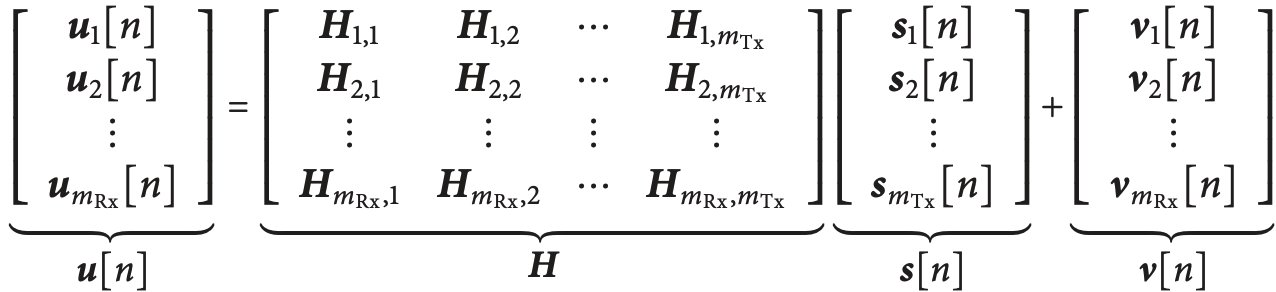
\includegraphics[width = 6.8cm]{img/wiener-multi.png}

  $\boldsymbol{H}_{i, j} \in \mathbb{C}^{M \times(M+K)}$ connects j-th transmitter to i-th receiver\\
  $\mathbf{H} \in \mathbb{C}^{M m_{\mathrm{Rx}} \times(M+K) m_{\mathrm{Tx}}}$\\
  $\boldsymbol{s}[n] \in \mathbb{C}^{(M+K) m_{\mathrm{Tx}}}$\\
  $\boldsymbol{v}[n] \in \mathbb{C}^{M m_{\mathrm{Rx}}}$\\
  $K$ is the maximum channel memory of all channels\\

  Main difference to before: Ordering of the elements in $\boldsymbol{s}[n]$ has changed to groups of time series.\\
  
  \textbf{Solution:}\\
  $$\boldsymbol{w}_{j, \mathrm{opt}}=\underbrace{\left(\boldsymbol{H} \boldsymbol{R}_{\boldsymbol{s}} \boldsymbol{H}^{\mathrm{H}}+\boldsymbol{R}_{v}\right)^{-1}}_{\boldsymbol{R}^{-1}} \underbrace{\boldsymbol{H} \boldsymbol{R}_{\boldsymbol{s}} \mathbf{e}_{(M+K)(j-1)+l_{j+1}}}_{\boldsymbol{p}}$$
  $$y_{j}[n]=\boldsymbol{w}_{j, \mathrm{opt}}^{\mathrm{H}} \boldsymbol{u}[n], \quad j \in\left\{1,2, \ldots, m_{\mathrm{Tx}}\right\}$$
  $\boldsymbol{w}_{j, \mathrm{opt}}$ is the optimum filter for recovering the signal of the j-th transmitter with time delay $l_j \in \{0,\dots,M+K-1\}$
\end{sectionbox}

\begin{sectionbox}
  \subsection{Kolmogorov-Wiener Filter for SISO}
  \textbf{Setup:}
  $$\boldsymbol{u} = \boldsymbol{h}s+\boldsymbol{v}, \quad \boldsymbol{s} = \boldsymbol{w}^H\boldsymbol{u}$$
  $$\boldsymbol{R}_{\boldsymbol{s}}=1, \quad \boldsymbol{R}_{v}=\mathbf{I},\quad s,v \text{ uncorrelated}$$
  \textbf{MSE solution:}
  $$\boldsymbol{w} = (\boldsymbol{I} + \boldsymbol{h}\boldsymbol{h}^H)^{-1}\boldsymbol{h} =\frac{\boldsymbol{h}}{1+\boldsymbol{h}^H\boldsymbol{h}}$$
\end{sectionbox}

\begin{sectionbox}
  \subsection{General Properties of Kolmogorov-Wiener}
  \begin{itemize}
    \item   Linear filter: can only use first order correlations of $d$ and $u$, $\quad\quad\quad\quad$ $\rightarrow$ $p$ must be $\neq 0$
    \item   Filtering without noise: MSE drops exponentially when increasing reconstruction filter length (if $\boldsymbol{H}$ has full column rank)
    \item   Filtering with noise: MSE saturates and cannot drop exponentially
  \end{itemize}
\end{sectionbox}

\begin{sectionbox}
  \subsection{Kolmogorov-Wiener Filter for SNR $\rightarrow \infty$}
  \textbf{Setup:}
  $$\boldsymbol{u} = \boldsymbol{H}\boldsymbol{s}+\boldsymbol{v}, \quad \hat{\boldsymbol{s}} = \boldsymbol{w}^H\boldsymbol{u}$$
  $$\boldsymbol{R}_{\boldsymbol{s}}=\sigma_{s}^{2} \mathbf{I}, \quad \boldsymbol{R}_{v}=\sigma_{v}^{2} \mathbf{I},\quad s,v \text{ uncorrelated}$$
  \textbf{MSE solution:}
  $$\begin{aligned}\lim _{\sigma_{s}^{2} / \sigma_{v}^{2} \rightarrow \infty} \boldsymbol{w}_{\mathrm{opt}}^{\mathrm{H}} &= \begin{cases}\mathbf{e}_{l+1}^{\mathrm{T}} \boldsymbol{H}^{\mathrm{H}}\left(\boldsymbol{H} \boldsymbol{H}^{\mathrm{H}}\right)^{-1}, & \text {full row rank } \boldsymbol{H} \\ \mathbf{e}_{l+1}^{\mathrm{T}}\left(\boldsymbol{H}^{\mathrm{H}} \boldsymbol{H}\right)^{-1} \boldsymbol{H}^{\mathrm{H}}, & \text {full column rank}\boldsymbol{H}\end{cases}\\&=\mathbf{e}_{l+1}^{\mathrm{T}} \boldsymbol{H}^{+}\end{aligned}$$

  Perfect reconstruction only if $H$ has full column rank:\\
  $$\hat{\boldsymbol{s}}_{l+1}=\mathbf{e}_{l+1}^{\mathrm{T}} \boldsymbol{H}^{+} \boldsymbol{H} \boldsymbol{s}=\mathbf{e}_{l+1}^{\mathrm{T}} \underbrace{\left(\boldsymbol{H}^{\mathrm{H}} \boldsymbol{H}\right)^{-1} \boldsymbol{H}^{\mathrm{H}} \boldsymbol{H}}_{\mathbf{I}} \boldsymbol{s}=\boldsymbol{s}_{l+1}$$

  Imperfect reconstruction if $H$ has not full column rank:\\
  $$\hat{s}_{l+1}=\mathbf{e}_{l+1}^{\mathrm{T}} \underbrace{\boldsymbol{H}^{+} \boldsymbol{H}}_{\neq \mathbf{I}} \boldsymbol{s} \neq \boldsymbol{s}_{l+}$$
  Because with $\operatorname{rank} \boldsymbol{H}<N$:\\
  $$\boldsymbol{H}^{+} \boldsymbol{H}=\mathbf{I}-\boldsymbol{P}_{\text {null } \boldsymbol{H}}$$
  $$\operatorname{dim} \text { null } \boldsymbol{H}=N-\operatorname{rank} \boldsymbol{H}>0$$
  $$\boldsymbol{P}_{\text {null } \boldsymbol{H}} \neq \mathbf{O}$$
\end{sectionbox}



\begin{sectionbox}
  \subsection{Steepest Descent Algorithm (SDA)}
  Kolmogorov-Wiener filters need to solve $\boldsymbol{R}\boldsymbol{w}_{\text{opt}} = \boldsymbol{p}$, where:\\
  $\boldsymbol{R}=\mathrm{E}\left[\boldsymbol{u}[n] \boldsymbol{u}^{\mathrm{H}}[n]\right]$ and $\boldsymbol{p}=\mathrm{E}\left[\boldsymbol{u}[n] d^{*}[n]\right]$\\
  Problems with solving explicitly
  \begin{itemize}
    \item Accuracy: computation of $m^2$ complex numbers for $R^{-1}$ and matrix vector multiplication add errors when $m$ is large 
    \item Computational load: Recomputing $R^{-1}$ at every time step is costly
    \item Gaussian elimination needs to restart the entire computation every time
    \item Triangular schemes bring no benefit as $R$ also changes
  \end{itemize}

  \textbf{Gradient of MSE}:\\
  $\operatorname{MSE}(w)=F\left(\frac{1}{2}\left(w+w^{\star}\right), \frac{1}{2}\left(w-w^{\star}\right) / \mathrm{j}\right)=G\left(w, w^{*}\right)$\\
  $\begin{aligned}\mathrm{dMSE}&=\left(\frac{\partial G}{\partial \boldsymbol{w}}\right)^{\mathrm{T}} \mathrm{d} \boldsymbol{w}+\left(\frac{\partial G}{\partial \boldsymbol{w}^{*}}\right)^{\mathrm{T}} \mathrm{d} \boldsymbol{w}^{*}\\&=\left(\frac{\partial G^{*}}{\partial \boldsymbol{w}^{*}}\right)^{\mathrm{H}} \mathrm{d} \boldsymbol{w}+\left(\left(\frac{\partial G}{\partial \boldsymbol{w}^{*}}\right)^{\mathrm{H}} \mathrm{d} \boldsymbol{w}\right)^{*}\\&=2 \operatorname{Re}\left\{\left(\frac{\partial G}{\partial w^{\star}}\right)^{\mathrm{H}} \mathrm{d} w\right\} = 2 \operatorname{Re}\left\{(\boldsymbol{R} w-\boldsymbol{p})^{\mathrm{H}} \mathrm{d} \boldsymbol{w}\right\}\\&\leq 2\left|(\boldsymbol{R} w-\boldsymbol{p})^{\mathrm{H}} \mathrm{d} \boldsymbol{w}\right|, \text{ with equality for } \mathrm{d} \boldsymbol{w}=(\boldsymbol{R} \boldsymbol{w}-\boldsymbol{p}) \mathrm{d} t\end{aligned}$\\
  

  \textbf{Gradient descent}:\\
  $$\boldsymbol{w}_{n+1}=\boldsymbol{w}_{n}-\left(\boldsymbol{R} \boldsymbol{w}_{n}-\boldsymbol{p}\right) \mu, \quad \mu>0$$
  $$\boldsymbol{w}_{n+1}=(\mathbf{I}-\mu \boldsymbol{R}) \boldsymbol{w}_{n}+\mu \boldsymbol{p}$$
  
  \textbf{Convergence}:\\
  $$\boldsymbol{c}_{n}=\boldsymbol{w}_{n}-\boldsymbol{w}_{\text {opt }}, \boldsymbol{c}_{n+1}=(\mathbf{I}-\mu \mathbf{R}) \boldsymbol{c}_{n}$$
  $$\boldsymbol{R}=\boldsymbol{Q}\boldsymbol{\Lambda}\boldsymbol{Q}^H, \boldsymbol{z}_{n}=\mathbf{Q}^{\mathrm{H}} \boldsymbol{c}_{n}, \boldsymbol{z}_{n+1}=(\mathbf{I}-\boldsymbol{\mu} \boldsymbol{\Lambda}) \boldsymbol{z}_{n}$$
  $$\Rightarrow \forall i \in\{1,2, \ldots, m\}: \left|1-\mu \lambda_{i}\right|<1 \Leftrightarrow 0< \mu < 2/\lambda_{\text{max}}$$
  sufficient (not necessary): $0<\mu<\frac{2}{\operatorname{tr} R}$\\ 
  
  \textbf{Steepest Descent Algorithm}:\\
  %$$\boldsymbol{w}_{n+1}=\boldsymbol{w}_{n}+\mu \boldsymbol{r}_{n}, \boldsymbol{r}_{n}=\boldsymbol{p}-\boldsymbol{R} \boldsymbol{w}_{n}, \mu_{\mathrm{opt}}=\frac{\boldsymbol{r}_{n}^{\mathrm{H}} \boldsymbol{r}_{n}}{\boldsymbol{r}_{n}^{\mathrm{H}} \boldsymbol{R} \boldsymbol{r}_{n}}$$ 
  $\mu_{\mathrm{opt}}$ is obtained by minimizing $\operatorname{MSE}_{n+1}$ wrt. $\mu$, i.e. $\frac{\partial \mathrm{MSE}_{n+1}}{\partial \mu^{*}} = 0$
  $\mathbf{M S E}_{n}=\boldsymbol{w}_{n}^{\mathrm{H}} \boldsymbol{R} \boldsymbol{w}_{n}-\boldsymbol{w}_{n}^{\mathrm{H}} \boldsymbol{p}-\boldsymbol{p}^{\mathrm{H}} \boldsymbol{w}_{n}+\sigma_{d}^{2}$\\
  $\boldsymbol{w}_{n+1}=\boldsymbol{w}_{n}+\mu \boldsymbol{r}_{n},\quad \boldsymbol{r}_{n} = \boldsymbol{p}-\boldsymbol{R}\boldsymbol{w}_{n}$\\
\end{sectionbox}
\begin{sectionbox}
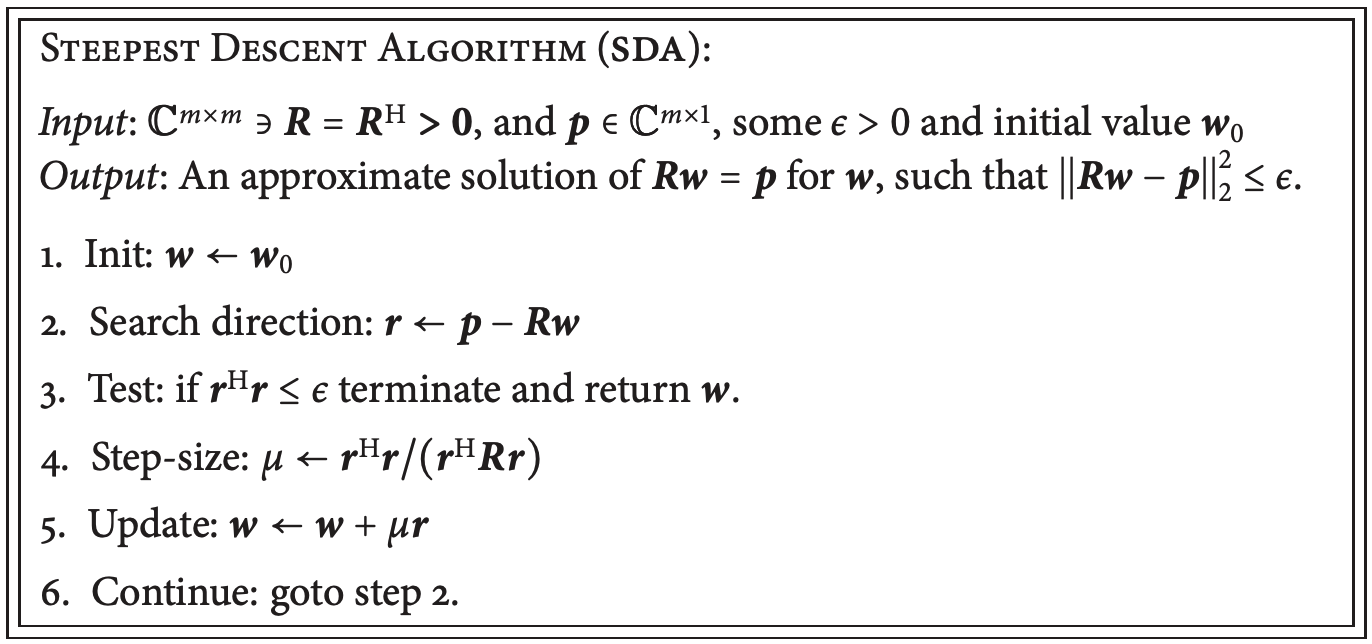
\includegraphics[width = 6.8cm]{img/sda.png}
Complexity: $M^{2} \log M$ scalar arithmetic operations/series time-steps\\
Complexity with full parallelization: $(\log M)^{2}$ time-steps\\
Steps 2-5 require $4m^2+5n-1$ scalar arithmetic operations per iteration\\
Number of iterations: $\approx 15(\operatorname{log}(M)-1), M > 15$
\end{sectionbox}

\begin{sectionbox}
  \subsection{SDA for constrained optimization}
  \textbf{Problem:}\\
  $$\min _{w} \boldsymbol{w}^{\mathrm{H}} \boldsymbol{A} \boldsymbol{w}, \quad \text { s.t. } \quad \boldsymbol{B}^{\mathrm{H}} \boldsymbol{w}=\boldsymbol{c}$$
  $$\mathbb{C}^{M \times M} \ni \boldsymbol{A}=\boldsymbol{A}^{\mathrm{H}}>\mathbf{0}, \boldsymbol{\boldsymbol{B}} \in \mathbb{C}^{M \times L}, \boldsymbol{c} \in \mathbb{C}^{L \times 1}, \text { rank } \boldsymbol{B}=L$$

  \textbf{Ansatz:}\\
  Decompose solution into fixed term $\boldsymbol{w}_{q}$ and variable term $\boldsymbol{z}$\\
  $$\boldsymbol{B}^{\mathrm{H}} \boldsymbol{w}_{\mathrm{q}}=\boldsymbol{c}, \quad \boldsymbol{z} \in \text { null } \boldsymbol{B}^{\mathrm{H}}$$
  $$\boldsymbol{w}=\boldsymbol{w}_{q}-\boldsymbol{z}$$
  Parameterize $\boldsymbol{z}$ by $\boldsymbol{w}_a$:
  $$\boldsymbol{B}=\underbrace{\left[\begin{array}{ll}
    \boldsymbol{U}_{1} & \boldsymbol{U}_{2}
    \end{array}\right]}_{\boldsymbol{U}}\left[\begin{array}{ll}
    \boldsymbol{\Sigma}_{1} & \mathbf{O} \\
    \mathbf{O} & \mathbf{O}
    \end{array}\right]\left[\begin{array}{l}
    \boldsymbol{V}_{1}^{\mathrm{H}} \\
    \boldsymbol{V}_{2}^{\mathrm{H}}
    \end{array}\right]$$
    $$\boldsymbol{z}=\boldsymbol{U}_{2} \boldsymbol{w}_{\mathrm{a}}, \quad \boldsymbol{w}_{\mathrm{a}} \in \mathbb{C}(M-L) \times 1 \Rightarrow \boldsymbol{z} \in \text{null}\boldsymbol{B}^H \forall \boldsymbol{w}_a$$
    
  Obtaining $\boldsymbol{U}_{2}$ without SVD:
  \begin{enumerate}
    \item Init: $\boldsymbol{U} \leftarrow\left[\begin{array}{ll}\boldsymbol{B} & \boldsymbol{F}\end{array}\right]$, where $\boldsymbol{F} \in \mathbb{C}^{M \times(M-L)}$ has i.i.d. random components.
    \item Orthogonalize with all yet orthogonalized columns.\\For $i=0$ to $M-1$:
    $$\boldsymbol{u}_{i} \leftarrow \boldsymbol{u}_{i}-\sum_{j=1}^{i-1} \boldsymbol{u}_{j}\left(\boldsymbol{u}_{j}^{\mathrm{H}} \boldsymbol{u}_{i}\right) /\left(\boldsymbol{u}_{j}^{\mathrm{H}} \boldsymbol{u}_{j}\right)$$
    \item Normalize: For $i \in\{L+1, L+2, \ldots M\}$ do $\boldsymbol{u}_{i} \leftarrow \boldsymbol{u}_{i} / \sqrt{\boldsymbol{u}_{i}^{\mathrm{H}} \boldsymbol{u}_{i}}$
    \item Output: $\boldsymbol{U}_{2} \leftarrow\left[\boldsymbol{u}_{L+1} \boldsymbol{u}_{L+2} \cdots \boldsymbol{u}_{M}\right] \in \mathbb{C}^{M \times(M-L)}$
  \end{enumerate}
  \vspace{0.2cm}
  Finding $w_q$ by SDA:\\
  $$w_{q}=\boldsymbol{B} \underbrace{\left(\boldsymbol{B}^{\mathrm{H}} \boldsymbol{B}\right)^{-1} c}_{q}$$
  $$\left(\boldsymbol{B}^{\mathrm{H}} \boldsymbol{B}\right) q=c$$
  $$w_{q}=\boldsymbol{B} q$$

  Reformulate:\\
  $$\min _{\boldsymbol{w}_{\mathrm{a}}}\left(\boldsymbol{w}_{\mathrm{q}}^{\mathrm{H}}-\boldsymbol{w}_{\mathrm{a}}^{\mathrm{H}} \boldsymbol{U}_{2}^{\mathrm{H}}\right) \boldsymbol{A}\left(\boldsymbol{w}_{\mathrm{q}}-\boldsymbol{U}_{2} \boldsymbol{w}_{\mathrm{a}}\right)$$

  \textbf{Solution:} run SDA with:\\
  $$\boldsymbol{R}=\boldsymbol{U}_{2}^{\mathrm{H}} \boldsymbol{A} \boldsymbol{U}_{2} \in \mathbb{C}^{(M-L) \times(M-L)}, \quad \text { and } \quad \boldsymbol{p}=\boldsymbol{U}_{2}^{\mathrm{H}} \boldsymbol{A} \boldsymbol{w}_{\mathrm{q}}$$
\end{sectionbox}

\begin{sectionbox}
  \subsection{Steepest Descent Procedure (SDP)}
  Problem: $R$ and $p$ are  unknown and need to be estimated.\\
  Drop assumption that $u[n]$ is WSS (e.g. channel changes) $\rightarrow$ $\boldsymbol{R}[n]$\\
  Estimation with exponential weighting:\\
  $$\widehat{\boldsymbol{R}}[n]=\frac{\sum_{k=0}^{\infty} \boldsymbol{u}[n-k] \boldsymbol{u}^{\mathrm{H}}[n-k] \alpha[k]}{\sum_{k=0}^{\infty} \alpha[k]}$$
  $$\alpha[k]= \begin{cases}1 & \text { for } k=0 \\ \eta^{k} & \text { for } k>0 \\ 0 & \text { else }\end{cases}, \sum_{k=0}^{\infty} \eta^{k}=\frac{1}{1-\eta}$$
  $$\widehat{\boldsymbol{R}}[n]=\eta \widehat{\boldsymbol{R}}[n-1]+(1-\eta) \boldsymbol{u}[n] \boldsymbol{u}^{\mathrm{H}}[n]$$
  $$\widehat{\boldsymbol{p}}[n]=\eta \widehat{\boldsymbol{p}}[n-1]+(1-\eta) \boldsymbol{u}[n] d^{*}[n]$$
  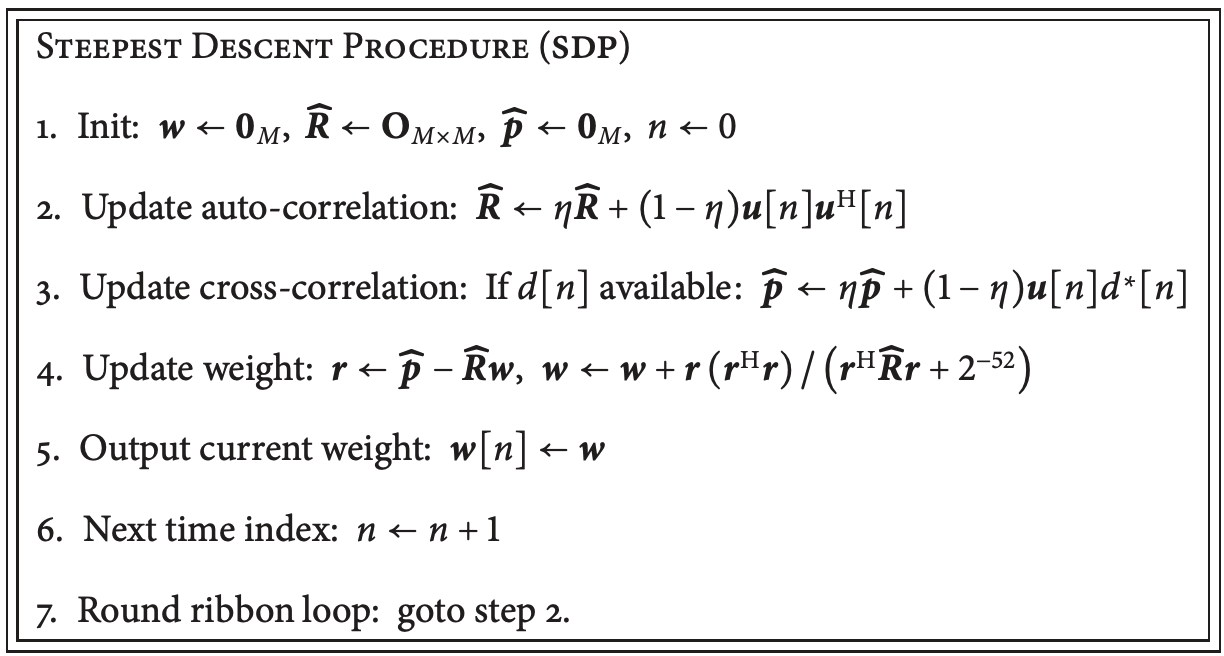
\includegraphics[width = 6.8cm]{img/sdp.png}
\end{sectionbox}

\begin{sectionbox}
  \subsection{SDP: Determining $\eta$}
  If $R[n]$ and $p[n]$ are changing slowly $\rightarrow$ choose $\eta$ close to 1\\
  If $R[n]$ and $p[n]$ remain const for $N_1$ time slots, but have completely changed after $N_2 > N_1$:\\
  $\eta^{N_{2}}=\gamma \ll 1$ and $\eta^{N_{1}}=1-\gamma$\\
  $\rightarrow$ $\eta=x^{1 / N_{1}}, \quad \text { where } \quad x^{N_{2} / N_{1}}+x-1=0, \quad 0<x<1$\\
  $N_{2} / N_{1}=30$ is a reasonable choice in practice $\rightarrow$ $\eta=\exp \left(-\frac{2.5}{N_{2}}\right)$\\

  \textbf{Radio Communications:}\\
  $N_2$ is the number of samples in which the receiver has moved by $\lambda$.
  For sample rate (bandwidth) $B$, wavelength $\lambda$, and speed $v$: $$\eta=\exp \left(-2.5 \frac{v}{B \lambda}\right)$$
\end{sectionbox}

\begin{sectionbox}
  \subsection{Least Mean Square (LMS)}
  Special Case of SDP for $\eta = 0$:
  $$\widehat{\boldsymbol{R}}[n]=\boldsymbol{u}[n] \boldsymbol{u}^{\mathrm{H}}[n], \quad \widehat{\boldsymbol{p}}[n]=\boldsymbol{u}[n] d^{*}[n]$$
  $$\mu=\frac{\boldsymbol{r}^{\mathrm{H}} \boldsymbol{r}}{\boldsymbol{r}^{\mathrm{H}} \widehat{\boldsymbol{R}} \boldsymbol{r}}=\frac{1}{\|\boldsymbol{u}[n]\|_{2}^{2}}$$
  $$\boldsymbol{r}=\widehat{\boldsymbol{p}}-\widehat{\boldsymbol{R}} \boldsymbol{w}=\boldsymbol{u}[n] (\underbrace{d^{*}[n]-\overbrace{\boldsymbol{u}^{\mathrm{H}}[n] \boldsymbol{w}}^{y^{*}[n]}}_{e^{*}[n]}) =\boldsymbol{u}[n] e^{*}[n]$$
  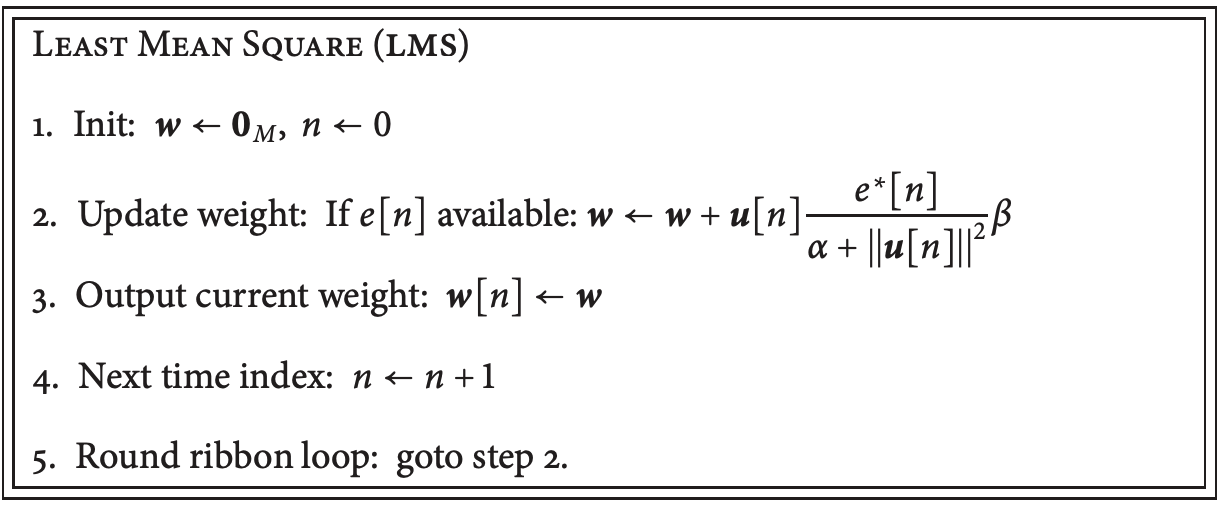
\includegraphics[width = 6.8cm]{img/lms.png}
  $\alpha > 0$: avoids very large step sizes, if $\boldsymbol{u}[n]$ is small\\
  $\beta > 0$: is for fine-tuning (found experimentally as well as $\alpha$)\\ 
\end{sectionbox}

\begin{sectionbox}
  \subsection{Block diagrams}
  Standard SDP and LMS:\\
  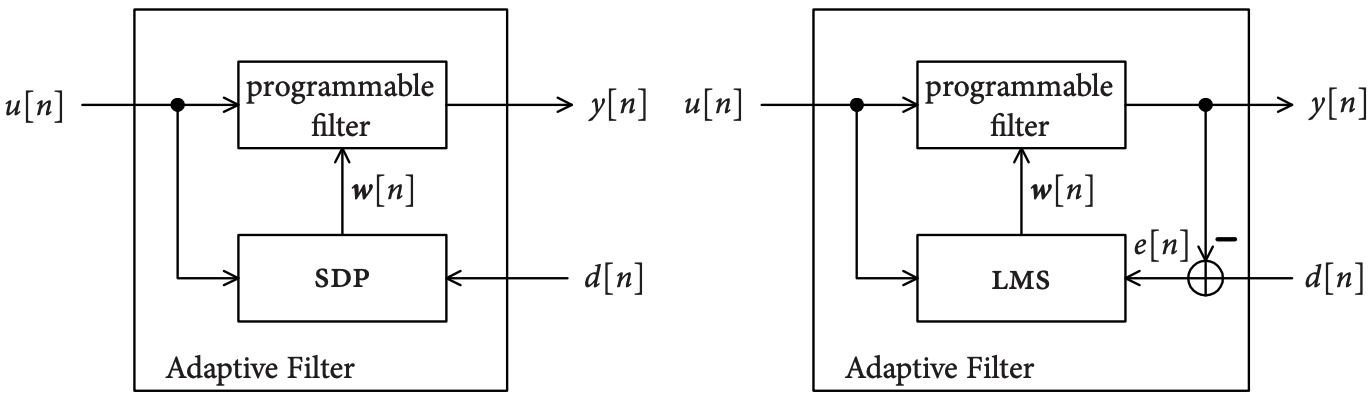
\includegraphics[width = 6.8cm]{img/blk-diagrams.png}\\
  Constrained SDP and LMS:
  $$z[n]=\boldsymbol{w}^{\mathrm{H}}[n] \boldsymbol{x}[n]$$
  $$\min _{w[n]} \mathrm{E}\left[|z[n]|^{2}\right], \quad \text { s.t. } \quad \boldsymbol{B}^{\mathrm{H}} \boldsymbol{w}[n]=\boldsymbol{c}$$
  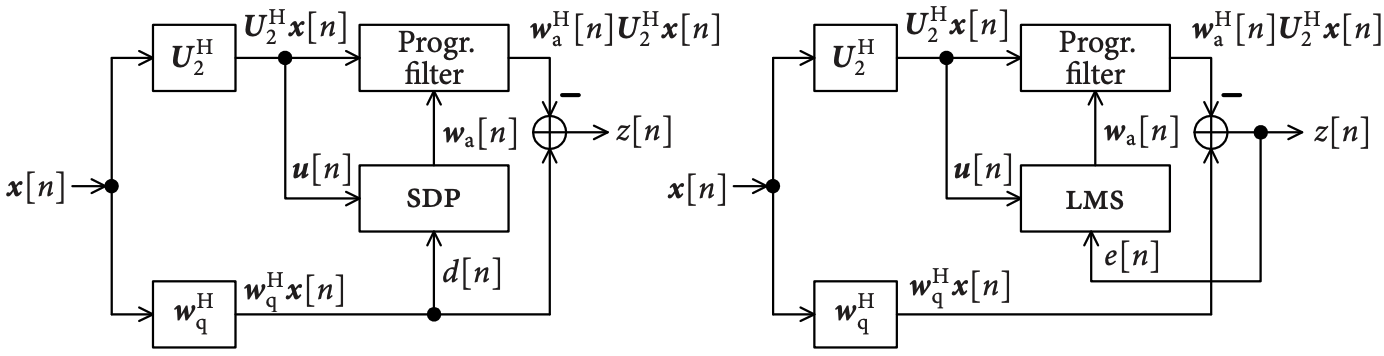
\includegraphics[width = 6.8cm]{img/blk-diagrams2.png}
  $$\boldsymbol{x}[n]=s_{i}[n] \boldsymbol{b}_{i} \quad \Longrightarrow \quad z[n]=s_{i}[n] c_{i}^{*}$$
  $$\boldsymbol{x}[n]\notin \operatorname{im} \boldsymbol{B} \quad \Longrightarrow \quad z[n]=0$$

\end{sectionbox}

\pagebreak
\section{Least Squares}
\begin{sectionbox}
  \subsection{Least Squares}
  Only $\boldsymbol{A}$ is known, no information about $\boldsymbol{\Upsilon}$ $\rightarrow$ ignore it all together\\
  \textbf{Least squares problem:}\\
  $$\boldsymbol{X} \approx \boldsymbol{A} \boldsymbol{S}$$
  $$\hat{\boldsymbol{S}}_{\mathrm{LS}}=\arg \min _{\boldsymbol{S}}\|\boldsymbol{X}-\boldsymbol{A S}\|_{\mathrm{F}}^{2}$$
  \textbf{Derivation:}
  $$\mathcal{E}=\|\boldsymbol{X}-\boldsymbol{A} \boldsymbol{S}\|_{\mathrm{F}}^{2}=\operatorname{tr}\left((\boldsymbol{X}-\boldsymbol{A} \boldsymbol{S})^{\mathrm{H}}(\boldsymbol{X}-\boldsymbol{A} \boldsymbol{S})\right)$$
  $$\frac{\partial \mathcal{E}}{\partial \boldsymbol{S}^{*}}=-\boldsymbol{A}^{\mathrm{H}} \boldsymbol{X}+\boldsymbol{A}^{\mathrm{H}} \boldsymbol{A} \boldsymbol{S} \leftarrow \frac{\partial \operatorname{tr}\left(\boldsymbol{S}^{\mathrm{H}} \boldsymbol{B}\right)}{\partial \boldsymbol{\boldsymbol{S}}^{*}} = \boldsymbol{B}$$

  \begin{emphbox}
    $\begin{aligned}
      \hat{\boldsymbol{S}}_{\mathrm{LS}} &=\left(\boldsymbol{A}^{\mathrm{H}} \boldsymbol{A}\right)^{-1} \boldsymbol{A}^{\mathrm{H}} \boldsymbol{X} \text{ (full column rank)}\\
      &=\boldsymbol{A}^{+} \boldsymbol{X} = \boldsymbol{A}^{+} \boldsymbol{A} \boldsymbol{S}+\boldsymbol{A}^{+} \boldsymbol{\Upsilon}\text{ (general)}
      \end{aligned}$
  \end{emphbox}
  $$\boldsymbol{A} \text { has full column rank } \Longrightarrow \hat{\boldsymbol{S}}_{\mathrm{LS}}=\boldsymbol{S}+\boldsymbol{A}^{+} \boldsymbol{\Upsilon}$$
  $$\mathrm{E}[\boldsymbol{\Upsilon}]=\mathbf{0}\Longrightarrow \text{ unbiased}$$
  Estimation noise:\\
  $$\mathrm{E}\left[\left\|\boldsymbol{A}^{+} \boldsymbol{\Upsilon}\right\|_{\mathrm{F}}^{2}\right] = \operatorname{tr}\left(\boldsymbol{A}^{+} \mathrm{E}\left[\boldsymbol{\Upsilon} \boldsymbol{\Upsilon}^{\mathrm{H}}\right] \boldsymbol{A}^{+\mathrm{H}}\right)$$
  For white noise $\mathrm{E}\left[\boldsymbol{\Upsilon} \boldsymbol{\Upsilon}^{\mathrm{H}}\right]=\mathbf{I}$ and full column rank $\boldsymbol{A}$:\\
  $$\mathrm{E}\left[\left\|\boldsymbol{A}^{+} \boldsymbol{\Upsilon}\right\|_{\mathrm{F}}^{2}\right] = \operatorname{tr}\left(\left(\boldsymbol{A}^{\mathrm{H}} \boldsymbol{A}\right)^{-1}\right) = \sum_{i} \frac{1}{\lambda_{i}},$$
  where $\lambda_i$ are the eigenvalues of $\boldsymbol{A}^H\boldsymbol{A}$ $\rightarrow$ minimal if all are the same\\

  For white observation noise the smallest possible variance is achieved iff:\\
  $$\boldsymbol{A}^{\mathrm{H}} \boldsymbol{A}=c \mathbf{I}, \quad \text { for any } c>0$$
  among all matrices $\boldsymbol{A} \in \mathbb{C}^{M \times d} \text { with }\|\boldsymbol{A}\|_{\mathrm{F}}^{2}=c$.
  \begin{itemize}
    \item $\boldsymbol{A}^{\mathrm{H}} \boldsymbol{A}$ has $\lambda_i = c/d$
    \item $\boldsymbol{A}$ must have orthogonal columns with the same euclidean norm
    \item use orthogonal pilot sequences
    \item purely deterministic approach, no need to know statistical properties
  \end{itemize}
\end{sectionbox}

\begin{sectionbox}
  \subsection{Pilot Sequence}
  \textbf{Setup:}
  $$\boldsymbol{u}=\boldsymbol{H}\boldsymbol{p}+\boldsymbol{v}\quad\Longleftrightarrow \quad\boldsymbol{u}=\boldsymbol{A} \boldsymbol{h}+\boldsymbol{v}$$
  $$\boldsymbol{A}=\left[\begin{array}{cccc}
    P_{0} & P_{1} & \cdots & P_{K} \\
    P_{1} & P_{2} & \cdots & P_{K+1} \\
    \vdots & \vdots & \vdots & \vdots \\
    P_{q-K-1} & P_{q-K} & \cdots & P_{q-1}
    \end{array}\right]$$
    $$\boldsymbol{h}=\left[\begin{array}{llll}
      h_{0} & h_{1} & \cdots & h_{K}
      \end{array}\right]^{\mathrm{T}}$$
      Necessary for full column rank: $q \geq 2 K+1$
\end{sectionbox}

\begin{sectionbox}
  \subsection{LS curve fitting}
  $$\hat{y}(x)=\frac{a}{x}+b+c x+d x^{2}+e x^{3}$$
  $$\underbrace{\left[\begin{array}{ccccc}
    1 / x_{1} & 1 & x_{1} & x_{1}^{2} & x_{1}^{3} \\
    1 / x_{2} & 1 & x_{2} & x_{2}^{2} & x_{2}^{3} \\
    \vdots & \vdots & \vdots & \vdots & \vdots \\
    1 / x_{N} & 1 & x_{N} & x_{N}^{2} & x_{N}^{3}
    \end{array}\right]}_{\boldsymbol{A}} \underbrace{\left[\begin{array}{c}
    a \\
    b \\
    c \\
    d \\
    e
    \end{array}\right]}_{\boldsymbol{w}} \approx \underbrace{\left[\begin{array}{c}
    y_{1} \\
    y_{2} \\
    \vdots \\
    y_{N}
    \end{array}\right]}_{\boldsymbol{y}}$$
    $$\boldsymbol{w}_{\mathrm{LS}}=\boldsymbol{A}^{+} \boldsymbol{y}$$
\end{sectionbox}


\begin{sectionbox}
  \subsection{Numerical integration with LS}
  Within every 3x3 window:
  $$\hat{f}(x, y)=a+b x^{2}+c y^{2}+d x^{2} y^{2}$$
  $$\left[\begin{array}{cccc}
    1 & h_{x}^{2} & h_{y}^{2} & h_{x}^{2} h_{y}^{2} \\
    1 & 0 & h_{y}^{2} & 0 \\
    \vdots & \vdots&\vdots&\vdots\\
    1 & h_{x}^{2} & h_{y}^{2} & h_{x}^{2} h_{y}^{2}
    \end{array}\right] \underbrace{\left[\begin{array}{c}
    a \\
    b \\
    c \\
    d
    \end{array}\right]}_{w} \approx\left[\begin{array}{c}
    f\left(-h_{x}, h_{y}\right) \\
    f\left(0, h_{y}\right) \\
    \vdots\\
    f\left(h_{x},-h_{y}\right)
    \end{array}\right]$$
    $$\hat{F}=\frac{4}{9} h_{x} h_{y}\left(9 a+3 b h_{x}^{2}+\left(3 c+d h_{x}^{2}\right) h_{y}^{2}\right)$$
    And without solving $w_{\mathrm{LS}}=\boldsymbol{A}^{+} \boldsymbol{f}$:
  $$\begin{aligned}
    \hat{F}=(& f\left(-h_{x}, h_{y}\right)+f\left(h_{x}, h_{y}\right)+f\left(-h_{x},-h_{y}\right)+f\left(h_{x},-h_{y}\right) \\
    &+4\left(f\left(0, h_{y}\right)+f\left(-h_{x}, 0\right)+f\left(h_{x}, 0\right)+f\left(0,-h_{y}\right)\right) \\
    &+16 f(0,0)) \frac{h_{x} h_{y}}{9}
    \end{aligned}$$
  3x3 window: quadratic convergence when increasing $M$\\
  5x5 window: cubic convergence when increasing $M$\\
  
  Procedure:\\
  $$F=\int_{y=y_{\min }}^{y_{\max }} \int_{x=x_{\min }}^{x_{\max }} f(x, y) \mathrm{d} x \mathrm{~d} y$$
  $$h_{x}=\frac{x_{\max }-x_{\min }}{M-1}, \quad h_{y}=\frac{y_{\max }-y_{\min }}{M-1}$$
  3x3 window: $ M \in\{3,5,7, \ldots\}$, 5x5 window: $M \in \{5,9,13, \ldots\}$\\
  
  Divide the integration region into $M$x$M$ parts. Move the local approximation by $3-1$, or $5-1$ grid points and sum up all.
  \begin{center}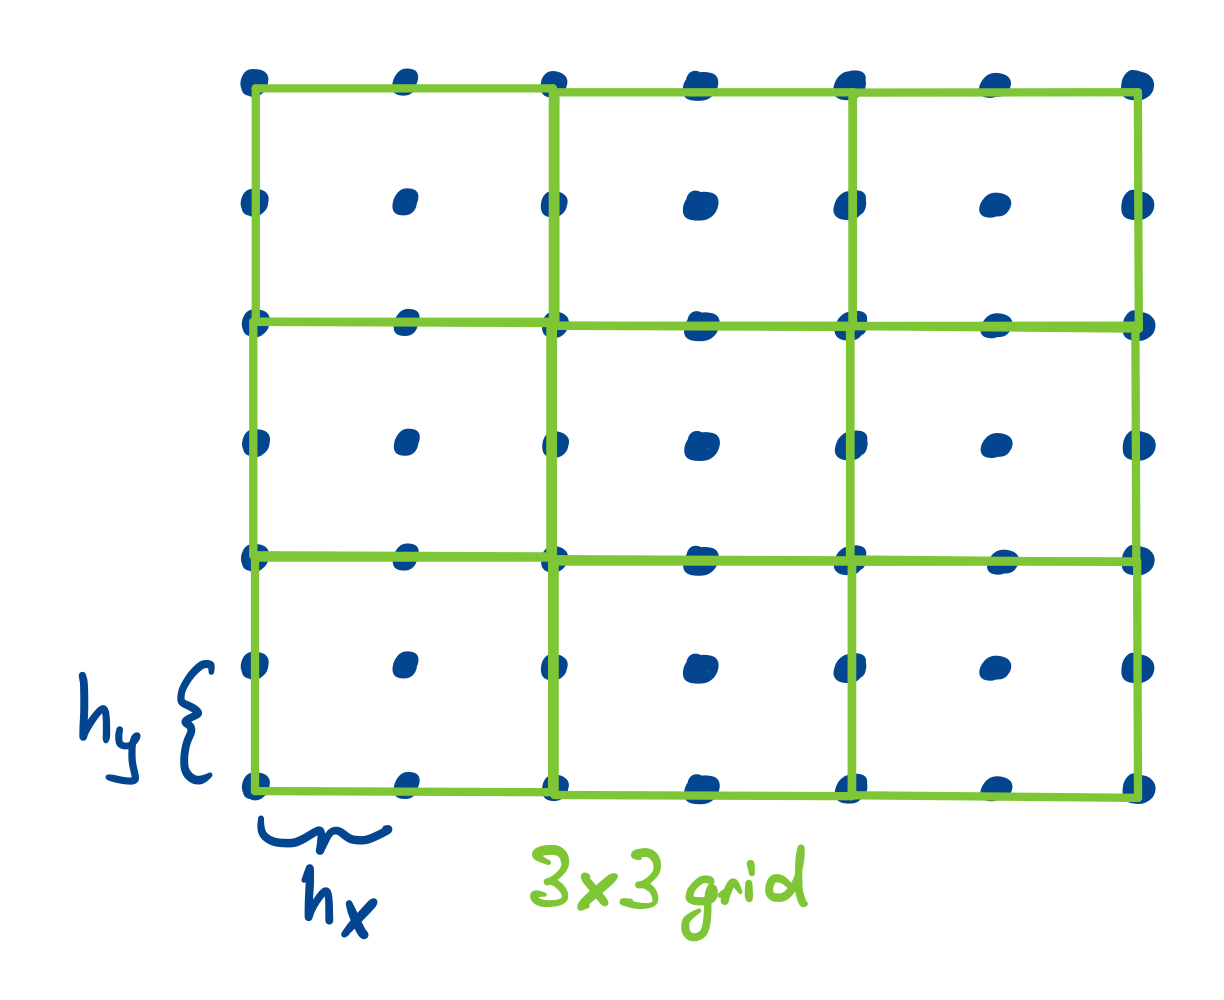
\includegraphics[width = 4cm]{img/grid2.jpeg}\end{center}
\end{sectionbox}

\begin{sectionbox}
  \subsection{Least squares as a projection}
  \textbf{Setup:}
  $$\boldsymbol{A} \boldsymbol{x}=\boldsymbol{b}, \quad \text { where } \quad \boldsymbol{b} \notin \operatorname{im} \boldsymbol{A}$$
  $$\boldsymbol{A} \boldsymbol{x}=\boldsymbol{b}+ \Delta\boldsymbol{b}, \quad \text { where } \quad \boldsymbol{b}+\Delta\boldsymbol{b} \in \operatorname{im} \boldsymbol{A}$$
  $$\Delta \boldsymbol{b}_{\mathrm{opt}}=\arg \min _{\Delta \boldsymbol{b}}\|\Delta \boldsymbol{b}\|_{2}^{2}, \quad \text { s.t. } \quad \boldsymbol{b}+\Delta \boldsymbol{b} \in \operatorname{im} \boldsymbol{A}$$
  Derivation:
  $$\Delta \boldsymbol{b}_{\mathrm{opt}}=\arg \min _{\Delta \boldsymbol{b}}\|\Delta \boldsymbol{b}\|_{2}^{2}, \quad \text { s.t. } \quad \boldsymbol{P}(\boldsymbol{b}+\boldsymbol{\Delta b})=\boldsymbol{b+\Delta b}$$
  $$\Delta \boldsymbol{b}_{\mathrm{opt}}=\arg \min _{\Delta \boldsymbol{b}}\|\Delta \boldsymbol{b}\|_{2}^{2}, \quad \text { s.t. } \quad(\mathbf{I}-\boldsymbol{P})(\boldsymbol{b}+\Delta \boldsymbol{b})=\mathbf{0}$$
  Lagrangian optimization yields:
  $$\Delta \boldsymbol{b}=-(\mathbf{I}-\boldsymbol{P}) \boldsymbol{b}$$
  \begin{emphbox}
    The least squares solution $\boldsymbol{x} = \boldsymbol{A}^+\boldsymbol{b}$ is the exact solution of $\boldsymbol{A}\boldsymbol{x} = \boldsymbol{P}\boldsymbol{b}$. I.e. the least squares estimation projects the measurements on $\operatorname{im}\boldsymbol{A}$\\
    $\boldsymbol{P} = \boldsymbol{A}\boldsymbol{A}^+$
  \end{emphbox}
\end{sectionbox}


\begin{sectionbox}
  \subsection{Total Least Squares}
  \textbf{Setup:}
  $$\min \left\|\left[\begin{array}{ll}
    \Delta \boldsymbol{A} & \Delta \boldsymbol{b}
  \end{array}\right]\right\|_{F}^{2} \quad\text{s.t.} \quad (\boldsymbol{A}+\Delta \boldsymbol{A}) \boldsymbol{x}=\boldsymbol{b}+\Delta \boldsymbol{b}$$

  Rewrite:
  $$\left[\begin{array}{ll}
    \boldsymbol{A} & b
    \end{array}\right]\left[\begin{array}{c}
    x \\
    -1
    \end{array}\right]=0, \quad \boldsymbol{b} \notin \operatorname{im} \boldsymbol{A}$$
  $\boldsymbol{b} \notin \operatorname{im} \boldsymbol{A}$, thus: $\operatorname{rank} [\boldsymbol{Ab}] = N + 1$ and $\operatorname{null} [\boldsymbol{Ab}] = \{0\}$\\
  $$\left[\begin{array}{ll}
    \boldsymbol{A} & \boldsymbol{b}
    \end{array}\right]=\boldsymbol{U} \boldsymbol{\Sigma} \boldsymbol{V}^{\mathrm{H}}=\sum_{k=1}^{N+1} s_{k} \boldsymbol{u}_{k} \boldsymbol{v}_{k}^{\mathrm{H}}$$

  Allow for solutions by increasing the dimensionality of the nullspace to 1:
    $$\left[\begin{array}{cc}
    \boldsymbol{A}+\Delta \boldsymbol{A} & \boldsymbol{b}+\Delta \boldsymbol{b}
    \end{array}\right]=\sum_{k=1}^{N} s_{k} \boldsymbol{u}_{k} \boldsymbol{v}_{k}^{\mathrm{H}}$$
  $$\left[\begin{array}{ll}
    \boldsymbol{A}+\Delta \boldsymbol{A} & \boldsymbol{b}+\Delta \boldsymbol{b}
    \end{array}\right] \boldsymbol{v}_{N+1} \alpha=\mathbf{0}$$
  
  The solution is optimal as we used the best approximation by Eckart-Young

  \begin{emphbox}
    $\boldsymbol{x}=\frac{-\left[\begin{array}{ll}
      \mathbf{I}_{N} & \mathbf{0}_{N}
      \end{array}\right] \boldsymbol{v}_{N+1}}{\left[\begin{array}{ll}
      \mathbf{0}_{N}^{\mathrm{T}} & 1
      \end{array}\right] \boldsymbol{v}_{N+1}}$
  \end{emphbox}
\end{sectionbox}

\section{BLUE}
\begin{sectionbox}
  \subsection{Best Linear Unbiased Estimator (BLUE)}
  $\boldsymbol{A}$ and $\mathrm{E}\left[\boldsymbol{\Upsilon} \boldsymbol{\Upsilon}^{\mathrm{H}}\right]$ are known\\
  \textbf{Setup:}
  $$\boldsymbol{X}=\boldsymbol{A} \boldsymbol{S}+\boldsymbol{\Upsilon}$$
  $$\boldsymbol{W}_{\text {BLUE }}=\arg \min _{\boldsymbol{W}} \mathrm{E}\left[\left\|\boldsymbol{W}^{\mathrm{H}} \boldsymbol{\Upsilon}\right\|_{\mathrm{F}}^{2}\right] \quad \text { s.t. } \quad \boldsymbol{W}^{\mathrm{H}} \boldsymbol{A}=\mathbf{I}$$
  $\rightarrow$ minimize estimation variance while being unbiased\\
  Derivation:
  $$\mathrm{E}\left[\left\|\boldsymbol{W}^{\mathrm{H}} \boldsymbol{\Upsilon}\right\|_{\mathrm{F}}^{2}\right] = \operatorname{tr}\left(W^{\mathrm{H}} \mathrm{E}\left[\boldsymbol{\Upsilon} \boldsymbol{\Upsilon}^{\mathrm{H}}\right] \boldsymbol{W}\right)$$
  $$\boldsymbol{W}^{\mathrm{H}} \boldsymbol{A}=\mathbf{I} \quad \Longleftrightarrow \quad \forall i: \boldsymbol{w}_{i}^{\mathrm{H}} \boldsymbol{A}=\mathbf{e}_{i}^{\mathrm{T}}$$
  Lagrangian optimization yields:
  \begin{emphbox}
    optimal weights:\\
    $\boldsymbol{W}_{\mathrm{BLUE}}=\left(\mathrm{E}\left[\boldsymbol{\Upsilon} \boldsymbol{\Upsilon}^{\mathrm{H}}\right]\right)^{-1} \boldsymbol{A}\left(\boldsymbol{A}^{\mathrm{H}}\left(\mathrm{E}\left[\boldsymbol{\Upsilon} \boldsymbol{\Upsilon}^{\mathrm{H}}\right]\right)^{-1} \boldsymbol{A}\right)^{-1}$\\
    minimal noise variance:\\
    $\mathrm{E}\left[\left\|\boldsymbol{W}_{\mathrm{BLUE}}^{\mathrm{H}} \boldsymbol{\Upsilon}\right\|_{\mathrm{F}}^{2}\right]=\operatorname{tr}\left(\left(\boldsymbol{A}^{\mathrm{H}}\left(\mathrm{E}\left[\boldsymbol{\Upsilon} \boldsymbol{\Upsilon}^{\mathrm{H}}\right]\right)^{-1} \boldsymbol{A}\right)^{-1}\right)$
  \end{emphbox}
  
  \textbf{Special case:} $\mathrm{E}\left[\boldsymbol{\Upsilon} \boldsymbol{\Upsilon}^{\mathrm{H}}\right]=\mathbf{I} \sigma_{v}^{2}$ white observation noise:
  $$\boldsymbol{W}_{\mathrm{BLUE}}^{\mathrm{H}}=\boldsymbol{A}^{+}=\boldsymbol{W}_{\mathrm{LS}}^{\mathrm{H}}$$
  \begin{itemize}
    \item noise must be colored in order for BLUE to improve the result
    \item $\boldsymbol{S}=0$ must be transmitted to estimate $\mathrm{E}\left[\boldsymbol{\Upsilon} \boldsymbol{\Upsilon}^{\mathrm{H}}\right]$ $\rightarrow$ extra payload
    \item if noise is WSS, $\mathrm{E}\left[\boldsymbol{\Upsilon} \boldsymbol{\Upsilon}^{\mathrm{H}}\right]$ can be estimated once
    \item if noise is not WSS: tradeoff between tracking performance and estimation error
  \end{itemize}
  

\end{sectionbox}


\begin{sectionbox}
  \subsection{BLUE for uncorrelated signal and noise}
\textbf{Special case:} noise and signal are uncorrelated:
\begin{emphbox}
  For $\mathrm{E}\left[\boldsymbol{S} \boldsymbol{\Upsilon}^{\mathrm{H}}\right] = 0$:\\
  $\boldsymbol{W}_{\text {BLUE }}=\left(\mathrm{E}\left[\boldsymbol{X} \boldsymbol{X}^{\mathrm{H}}\right]\right)^{-1} \boldsymbol{A}\left(\boldsymbol{A}^{\mathrm{H}}\left(\mathrm{E}\left[\boldsymbol{X} \boldsymbol{X}^{\mathrm{H}}\right]\right)^{-1} \boldsymbol{A}\right)^{-1}$
\end{emphbox}

If the statistics are unknown, they can be estimated using the observation matrix $\boldsymbol{X}$:
$$\widehat{\boldsymbol{W}}_{\mathrm{BLUE}}=\left(\boldsymbol{X} \boldsymbol{X}^{\mathrm{H}}\right)^{-1} \boldsymbol{A}\left(\boldsymbol{A}^{\mathrm{H}}\left(\boldsymbol{X} \boldsymbol{X}^{\mathrm{H}}\right)^{-1} \boldsymbol{A}\right)^{-1}$$
\begin{itemize}
  \item no need to switch of signal for estimating the noise variance
  \item if noise is WSS: estimation is easy (once)
  \item if noise is not WSS: tradeoff between estimation error and tracking performance
  \item $XX^H$ must be invertible $\rightarrow$ needs enough samples 
  \item loss of generality
  \item latency: samples $\boldsymbol{X}$ have to be gathered before estimation can start (LS can start immideately)
\end{itemize}
\end{sectionbox}

\begin{sectionbox}
  \subsection{BLUE for multi-user detection}
  \textbf{General Setup:}\\
  Q users with signals $\tilde{\boldsymbol{S}}_i$ and full column rank channels $\tilde{H}_i$, additive white noise, signals $S_i$ and $S_j$ are uncorrelated for $i\neq j$
  $$\boldsymbol{X}=\sum_{i=1}^{Q} \tilde{\boldsymbol{H}}_{i} \tilde{\boldsymbol{S}}_{i}+\boldsymbol{\Theta}, \quad \mathrm{E}\left[\boldsymbol{\Theta}\boldsymbol{\Theta}^{\mathrm{H}}\right]=\mathbf{I},\quad \mathrm{E}\left[\tilde{\boldsymbol{S}}_{i} \tilde{\boldsymbol{S}}_{i}^{\mathrm{H}}\right]=\sigma_{i}^{2} \mathbf{I}$$  
  \textbf{Normalized Setup:} $\boldsymbol{H}_{i}=\tilde{\boldsymbol{H}}_{i} \sigma_{i}, \quad \text { and } \quad \boldsymbol{S}_{i}=\tilde{\boldsymbol{S}}_{i} / \sigma_{i}$\\
  $$\boldsymbol{X}=\sum_{i=1}^{Q} \boldsymbol{H}_{i} \boldsymbol{S}_{i}+\boldsymbol{\Theta},\quad \mathrm{E}\left[\boldsymbol{\Theta} \boldsymbol{\Theta}^{\mathrm{H}}\right]=\mathbf{I}, \quad \mathrm{E}\left[\boldsymbol{S}_{i} \boldsymbol{S}_{i}^{\mathrm{H}}\right]=\mathrm{I}$$
  For reconstructing the signal of the k-th user:
  $$\boldsymbol{X}=\boldsymbol{H}_{k} \boldsymbol{S}_{k}+\underbrace{\sum_{i=1, i \neq k}^{Q} \boldsymbol{H}_{i} \boldsymbol{S}_{i}+\boldsymbol{\Theta}}_{\boldsymbol{\Upsilon}_{k}}=\boldsymbol{H}_{k} \boldsymbol{S}_{k}+\boldsymbol{\Upsilon}_{k}$$
  Solution for the BLUE:
  $$\boldsymbol{W}_{k}=\left(\mathrm{E}\left[\boldsymbol{X} \boldsymbol{X}^{\mathrm{H}}\right]\right)^{-1} \boldsymbol{H}_{k}\left(\boldsymbol{H}_{k}^{\mathrm{H}}\left(\mathrm{E}\left[\boldsymbol{X} \boldsymbol{X}^{\mathrm{H}}\right]\right)^{-1} \boldsymbol{H}_{k}\right)^{-1}$$
  $$\mathrm{E}\left[\boldsymbol{X} \boldsymbol{X}^{\mathrm{H}}\right]=\mathbf{I}+\sum_{i=1}^{Q} \boldsymbol{H}_{i} \boldsymbol{H}_{i}^{\mathrm{H}}$$
  Procedure for estimating all signals:\\
  1. Find the signal with the lowest estimation noise, by computing all noises and finding the minimum
  $$\begin{aligned}\xi_{k}&=\mathrm{E}\left[\left\|\boldsymbol{W}_{k}^{\mathrm{H}} \boldsymbol{\Upsilon}_{k}\right\|_{\mathrm{F}}^{2}\right]\\&=\operatorname{tr}\left(\boldsymbol{W}_{k}^{\mathrm{H}}\left(\mathbf{I}+\sum_{i=1, i \neq k}^{Q} \boldsymbol{H}_{i} \boldsymbol{H}_{i}^{\mathrm{H}}\right) \boldsymbol{W}_{k}\right)\end{aligned}$$
  $$k_{*}=\arg \min _{k \in\{1,2, \ldots Q\}} \xi_{k}$$
  2. compute the estimated signal and subtract it from the observation
  $$\hat{\boldsymbol{S}}_{k_{*}}=\boldsymbol{W}_{k_{\star}}^{\mathrm{H}} \boldsymbol{X}$$
  $$\boldsymbol{X} \leftarrow \boldsymbol{X}-\boldsymbol{H}_{k_{*}} \boldsymbol{S}_{k_{*}}$$
  3. repeat the procedure with the remaining measurement

  \begin{itemize}
    \item BLUE usually does not yield the minimum MSE (also unbiased)
    \item optimum filter wrt. MSE is given by: ($\mathrm{E}[\|\boldsymbol{W}^{\mathrm{H}} \boldsymbol{X}-\boldsymbol{S}\|_{\mathrm{F}}^{2}]$)
  \end{itemize}
  $$\boldsymbol{W}_{\mathrm{opt}}=\left(\mathrm{E}\left[\boldsymbol{X} \boldsymbol{X}^{\mathrm{H}}\right]\right)^{-1} \mathrm{E}\left[\boldsymbol{X} \boldsymbol{S}^{\mathrm{H}}\right]$$
\end{sectionbox}

\section{MUSIC}
\begin{sectionbox}
  \subsection{MUSIC: Multiple Signal Classification}
  Nothing is known except for algebraic structure\\
  \textbf{Setup and restrictions:}
  $$\boldsymbol{X}=\boldsymbol{A} \boldsymbol{S}+\boldsymbol{\Upsilon}$$
  $$\boldsymbol{A}=\left[\begin{array}{llll}
    \boldsymbol{a}\left(\theta_{1}\right) & \boldsymbol{a}\left(\theta_{2}\right) & \cdots & \boldsymbol{a}\left(\theta_{d}\right)
    \end{array}\right] \in \mathbb{C}^{M \times d}$$
    $$\boldsymbol{a}(\theta)=\left[\begin{array}{c}
      a_{1}(\theta) \\
      a_{2}(\theta) \\
      \vdots \\
      a_{M}(\theta)
      \end{array}\right]$$
  
  $$\operatorname{rank}\left(\boldsymbol{S} \in \mathbb{C}^{d \times N}\right)=d,  \quad \operatorname{rank}(\boldsymbol{A})=d, d<M$$
$$\theta_{1}, \theta_{2}, \ldots, \theta_{M} \text { pairwise different }$$
$$\Downarrow$$
$$\left(\begin{array}{llll}
  \boldsymbol{a}\left(\theta_{1}\right) & \boldsymbol{a}\left(\theta_{2}\right) & \cdots & \boldsymbol{a}\left(\theta_{M}\right)
  \end{array}\right) \text { are linearly independent }$$

\textbf{Goal:} find $d$, $\theta_i$, and $\boldsymbol{S}$\\
\textbf{Derivation without noise:}
$$\operatorname{im}(\boldsymbol{A})=\operatorname{im}\left(\boldsymbol{A} \boldsymbol{S} \boldsymbol{S}^{\mathrm{H}} \boldsymbol{A}^{\mathrm{H}}\right)$$
$$\boldsymbol{X}\boldsymbol{X}^H = \boldsymbol{A \boldsymbol{S} \boldsymbol{S}}^{\mathrm{H}} \boldsymbol{A}^{\mathrm{H}}=[\underbrace{\boldsymbol{u}_{1} \cdots \boldsymbol{u}_{d}}_{\boldsymbol{U}_{1}} \underbrace{\boldsymbol{u}_{d+1} \cdots \boldsymbol{u}_{M}}_{\boldsymbol{U_2}}]
\boldsymbol{\Lambda} \boldsymbol{U}^{\mathrm{H}}$$
$$\lambda_{1} \geq \lambda_{2} \geq \cdots \geq \lambda_{d}>0$$
$$\operatorname{im}(\boldsymbol{A})=\operatorname{im}\left(\boldsymbol{U}_{1}\right) \rightarrow
y \in \operatorname{im}(\boldsymbol{A}) \Longleftrightarrow \quad \boldsymbol{U}_{2}^{\mathrm{H}} \boldsymbol{y}=0$$
$$\forall i \in\{1,2, \ldots, d\}: \quad \boldsymbol{U}_{2}^{\mathrm{H}} \boldsymbol{a}\left(\theta_{i}\right)=\mathbf{0}$$

In summary:
\begin{emphbox}
  $\left\|\boldsymbol{U}_{2}^{\mathrm{H}} \boldsymbol{a}(\theta)\right\|_{2}^{2} \begin{cases}=0 & \text { for } \theta \in\left\{\theta_{1}, \theta_{2}, \ldots, \theta_{d}\right\} \\ >0 & \text { else. }\end{cases}$
\end{emphbox}

\textbf{Modification with noise:}
$$\mathrm{E}\left[\boldsymbol{\Upsilon} \boldsymbol{\Upsilon}^{\mathrm{H}}\right]=\sigma_{\Upsilon}^{2} \mathbf{I}, \quad \text { and } \quad \mathrm{E}\left[\boldsymbol{S} \boldsymbol{\Upsilon}^{\mathrm{H}}\right]=\mathbf{O}$$

$\mathrm{E}\left[\boldsymbol{X} \boldsymbol{X}^{\mathrm{H}}\right]$
$$= [\boldsymbol{U}_1 \boldsymbol{U}_2] \operatorname{diag}(\lambda_1+\sigma_{\Upsilon}^2, \dots, \lambda_d+\sigma_{\Upsilon}^2,\sigma_{\Upsilon}^2,\dots,\sigma_{\Upsilon}^2)[\boldsymbol{U}_1 \boldsymbol{U}_2]^H$$

Approximation:
$$\boldsymbol{X}\boldsymbol{X}^H = [\hat{\boldsymbol{U}}_1 \hat{\boldsymbol{U}}_2]\operatorname{diag}(\hat{\lambda}_1,\dots,\hat{\lambda}_M)[\hat{\boldsymbol{U}}_1 \hat{\boldsymbol{U}}_2]^H$$
For determining $d$, find the last significant drop in $\hat{\lambda}_i$.\\

\textbf{MUSIC spectrum:} has maxima close to $\theta_i$
\begin{emphbox}
  $F(\theta)=\frac{\|\boldsymbol{a}(\theta)\|_{2}^{2}}{\left\|\widehat{\boldsymbol{U}}_{2}^{\mathrm{H}} \boldsymbol{a}(\theta)\right\|_{2}^{2}}$
\end{emphbox}


Procedure:
\begin{enumerate}
  \item Compute eigenvalue decomposition of $XX^H$
  \item Scan eigenvalues for jumps and determine $\hat{d}$
  \item Find locations $\hat{\theta}_i$ at $\hat{d}$ strongest peaks of the MUSIC spectrum $F(\theta)$
  \item Form the matrix $\widehat{\boldsymbol{A}}=\left[\begin{array}{llll}
    \boldsymbol{a}\left(\widehat{\theta}_{1}\right) & \boldsymbol{a}\left(\widehat{\theta}_{2}\right) & \cdots & \boldsymbol{a}\left(\widehat{\theta}_{\widehat{d}}\right)
    \end{array}\right]$
  \item Solve for $\hat{\boldsymbol{S}}$ with pseudo-inverse $\hat{\boldsymbol{S}} = \hat{\boldsymbol{A}}^+\boldsymbol{X}$
\end{enumerate}


\end{sectionbox}
\begin{sectionbox}
  Signal-to-noise ratio:
  $$\operatorname{SNR} = \frac{\mathrm{E}\left[\|\boldsymbol{A} \boldsymbol{S}\|_{\mathrm{F}}^{2}\right]}{\mathrm{E}\left[\|\boldsymbol{\Upsilon}\|_{\mathrm{F}}^{2}\right]}$$
  
  Maximum number of signals:\\
  At most $d = M-1$ complex components can be resolved $\rightarrow$ $\boldsymbol{U}_2$ does not exist for larger $d$. Otherwise, $M$ has to be increased by either lowering $N$ or increasing the number if samples.\\

  Sharpness of the peaks:\\
  The peaks get sharper when $N$ is increased $\rightarrow \hat{\boldsymbol{U}}_2$ more accurate. The higher $N$, the closer targets can be resolved.

  \textbf{MUSIC with colored noise:}
$$\begin{aligned}
  \boldsymbol{X}^{\prime} &=\left(\mathrm{E}\left[\boldsymbol{\Upsilon} \boldsymbol{\Upsilon}^{\mathrm{H}}\right]\right)^{-1 / 2} \boldsymbol{X} \\
  &=\underbrace{\left(\mathrm{E}\left[\boldsymbol{\Upsilon} \boldsymbol{\Upsilon}^{\mathrm{H}}\right]\right)^{-1 / 2} \boldsymbol{A}}_{\boldsymbol{A}^{\prime}} \boldsymbol{S}+\underbrace{\left(\mathrm{E}\left[\boldsymbol{\Upsilon} \boldsymbol{\Upsilon}^{\mathrm{H}}\right]\right)^{-1 / 2} \boldsymbol{\Upsilon}}_{\boldsymbol{\Upsilon}^{\prime}} \\
  &=\boldsymbol{A}^{\prime} \boldsymbol{S}+\boldsymbol{\Upsilon}^{\prime} .
  \end{aligned}$$
\end{sectionbox}
\begin{sectionbox}
  \subsection{MUSIC for multiple frequency estimation}
  \textbf{Setup:}
  $$\boldsymbol{a}\left(\omega_{i}\right)=\left[\begin{array}{c}
    1 \\
    \mathrm{e}^{\mathrm{j} \omega_{i} T} \\
    \mathrm{e}^{\mathrm{j} 2 \omega_{i} T} \\
    \vdots \\
    \mathrm{e}^{\mathrm{j}(M-1) \omega_{i} T}
    \end{array}\right]$$
  $$x[n]=\sum_{i=1}^{d} c_{i} \mathrm{e}^{\mathrm{j} \omega_{i} T n}$$
  $$\boldsymbol{x}[n]=\left[\begin{array}{c}
    x[n] \\
    x[n+1] \\
    x[n+2] \\
    \vdots \\
    x[n+M-1]
    \end{array}\right]=\sum_{i=1}^{d}\left[\begin{array}{c}
    c_{i} \mathrm{e}^{\mathrm{j} \omega_{i} T n} \\
    c_{i} \mathrm{e}^{\mathrm{j} \omega_{i} T(n+1)} \\
    c_{i} \mathrm{e}^{\mathrm{j} \omega_{i} T(n+2)} \\
    \vdots \\
    c_{i} \mathrm{e}^{\mathrm{j} \omega_{i} T(n+M-1)}
    \end{array}\right]$$
  $$=\underbrace{\left[\begin{array}{lll}
    \boldsymbol{a}\left(\omega_{1}\right)  & \cdots & \boldsymbol{a}\left(\omega_{d}\right)
    \end{array}\right]}_{\boldsymbol{A}} \underbrace{\left[\begin{array}{c}
    c_{1} \mathrm{e}^{\mathrm{j} \omega_{1} T n} \\
    c_{2} \mathrm{e}^{\mathrm{j} \omega_{2} T n} \\
    \vdots \\
    c_{d} \mathrm{e}^{\mathrm{j} \omega_{d} T n}
    \end{array}\right]}_{\boldsymbol{s}[n]}=\boldsymbol{A} \boldsymbol{s}[n]$$
  $$\boldsymbol{X}=\left[\begin{array}{llll}
    \boldsymbol{x}[n] & \boldsymbol{x}[n+1] & \cdots & \boldsymbol{x}[n+N-1]
    \end{array}\right]$$

  $\boldsymbol{A}$ is Vandermode  $\rightarrow$ for pairwise different $\theta_i$, the columns of $\boldsymbol{A}$ are LI

\end{sectionbox}



\begin{sectionbox}
  \subsection{Sampling of plane waves}
  $$p(t, \overrightarrow{\boldsymbol{r}})=P(t-\overrightarrow{\boldsymbol{\kappa}} \cdot \overrightarrow{\boldsymbol{r}} / c)$$
  $\overrightarrow{\boldsymbol{\kappa}}$: direction unit vector, $c$: propagation speed\\
  Harmonic planar wave:
  $$p(t, \vec{r})=A \cos \left(\omega_{0} t-k_{0} \overrightarrow{\boldsymbol{\kappa}} \cdot \overrightarrow{\boldsymbol{r}}+\varphi\right), k_{0}=\omega_{0} / c=2 \pi f_{0} / c$$

  Modulated harmonic planar wave:
  $$p(t, \overrightarrow{\boldsymbol{r}})=A(t-\overrightarrow{\boldsymbol{\kappa}} \cdot \overrightarrow{\boldsymbol{r}} / c) \cos \left(\omega_{0} t-k_{0} \overrightarrow{\boldsymbol{\kappa}} \cdot \overrightarrow{\boldsymbol{r}}+\varphi(t-\overrightarrow{\boldsymbol{\kappa}} \cdot \overrightarrow{\boldsymbol{r}} / c)\right)$$
  If changes occur only slowly in time (approx. constant withing one period):\\
  $A\left(t-\lambda_{0} / c\right)=A\left(t-1 / f_{0}\right) \approx A(t)$ \\
  $\varphi\left(t-\lambda_{0} / c\right)=\varphi\left(t-1 / f_{0}\right) \approx \varphi(t)$
  $$p\left(t, \overrightarrow{\boldsymbol{r}}+\overrightarrow{\boldsymbol{\kappa}} \lambda_{0}\right)=p(t, \overrightarrow{\boldsymbol{r}})$$

  Short notation with complex numbers: 
$$s(t, \overrightarrow{\boldsymbol{r}})=A(t-\overrightarrow{\boldsymbol{\kappa}} \cdot \overrightarrow{\boldsymbol{r}} / c) \mathrm{e}^{-\mathrm{j} k_{0} \overrightarrow{\boldsymbol{\kappa}} \cdot \overrightarrow{\boldsymbol{r}}+\mathrm{j} \varphi(t-\overrightarrow{\boldsymbol{\kappa}} \cdot \overrightarrow{\boldsymbol{r}} / c)}$$
$$p(t, \overrightarrow{\boldsymbol{r}})=\operatorname{Re}\left\{s(t, \overrightarrow{\boldsymbol{r}}) \mathrm{e}^{\mathrm{j} \omega_{0} t}\right\}$$

  After modulating to the baseband and filtering with a LP:
%$$s(n T, \vec{r})=\left.\left(h_{\mathrm{LPF}}(t) \star\left(2 p(t, \vec{r}) \mathrm{e}^{-\mathrm{j} \omega_{0} t}\right)\right)\right|_{t=n T+\tau_{\mathrm{LPF}}}$$
$$\boldsymbol{x}[n]=\left[\begin{array}{c}
  s\left(n T, \overrightarrow{\boldsymbol{r}}_{0}\right) \\
  s\left(n T, \overrightarrow{\boldsymbol{r}}_{1}\right) \\
  \vdots \\
  s\left(n T, \overrightarrow{\boldsymbol{r}}_{M-1}\right)
  \end{array}\right]$$

If sampling points are close together: $\forall i: \quad\left|\overrightarrow{\boldsymbol{r}}_{i}\right| \ll c T,$ ($cT/30$)\vspace{-0.1cm}
$$\begin{aligned}x[n]&=\underbrace{A(n T) \mathrm{e}^{j \varphi(n T)} \mathrm{e}^{j \psi}}_{s[n]} \overbrace{\left[\begin{array}{l}
  \mathrm{e}^{-j\left(k_{0} \overrightarrow{\boldsymbol{\kappa}} \cdot \overrightarrow{\boldsymbol{r}}_{0}+\psi\right)} \\
  \mathrm{e}^{-j\left(k_{0} \overrightarrow{\boldsymbol{\kappa}} \cdot \overrightarrow{\boldsymbol{r}}_{1}+\psi\right)} \\
  \vdots \\
  \mathrm{e}^{-j\left(k_{0} \overrightarrow{\boldsymbol{\kappa}} \cdot \overrightarrow{\boldsymbol{r}}_{M-1}+\psi\right)}
  \end{array}\right]}^{\boldsymbol{a}(\overrightarrow{\boldsymbol{\kappa}})}\\&=s[n] \boldsymbol{a}(\overrightarrow{\boldsymbol{\kappa}})\end{aligned}$$
  The angle $\psi$ is arbitrary as it cancels out $\rightarrow$ used for simplifying
\end{sectionbox}

\begin{sectionbox}
  \subsection{MUSIC for DOA estimation using ULAs}
  M sensors on a line with constant distance $\delta$ along the z-axis:
  $$\overrightarrow{\boldsymbol{r}}_{i}=\left(\frac{1}{2}(M-1)-i\right) \delta \overrightarrow{\mathbf{e}}_{z}, \quad i \in\{0,1, \ldots, M-1\}$$
  $$\overrightarrow{\boldsymbol{\kappa}}=-\cos (\phi) \sin (\theta) \mathbf{e}_{x}-\sin (\phi) \sin (\theta) \mathbf{e}_{y}-\cos (\theta) \mathbf{e}_{z}$$
  The angle is measured from the side of the ULA.
  The steering vector becomes:
  $$\boldsymbol{a}(\theta)=\left[\begin{array}{c}
    1 \\
    \mathrm{e}^{-\mathrm{j} k_{0} \delta \cos \theta} \\
    \mathrm{e}^{-2 \mathrm{j} k_{0} \delta \cos \theta} \\
    \vdots \\
    \mathrm{e}^{-(M-1) j k_{0} \delta \cos \theta}
    \end{array}\right]$$
  with
  $$\psi=\frac{1}{2}(M-1) k_{0} \delta \cos \theta$$
  spacial normalized angular frequency:
  $$\mu=-k_{0} \delta \cos \theta=-2 \pi \frac{\delta}{\lambda_{0}} \cos \theta$$
  $$\boldsymbol{a}(\mu)=\left[\begin{array}{c}
    1 \\
    \mathrm{e}^{\mathrm{j} \mu} \\
    \mathrm{e}^{\mathrm{j} 2 \mu} \\
    \vdots \\
    \mathrm{e}^{\mathrm{j}(M-1) \mu}
    \end{array}\right]$$
aliasing:
    $$\boldsymbol{a}(\mu)=\boldsymbol{a}(\mu+2 \pi n), \quad n \in\{\pm 1, \pm 2, \cdots\}$$
    $$\text { no directional aliasing } \Longleftrightarrow \quad k_{0} \delta<\pi \quad \Longleftrightarrow \quad \delta<\lambda_{0} / 2$$

    If $0^{\circ}$ is chosen to be orthogonal to the ULA and measured from the center to the right:
    $$\boldsymbol{a}(\theta)=\left[\begin{array}{c}
      1 \\
      \mathrm{e}^{-\mathrm{j} k_{0} \delta \sin \theta} \\
      \mathrm{e}^{-2 \mathrm{j} k_{0} \delta \sin \theta} \\
      \vdots \\
      \mathrm{e}^{-(M-1) j k_{0} \delta \sin \theta}
      \end{array}\right]$$
\end{sectionbox}

\begin{sectionbox}
  \subsection{Useful identities}
  $$1+z+z^2+\dots+z^{M-1} = \frac{z^M - 1}{z-1}$$
  $$z^M - 1 = 0\Leftrightarrow z = e^{j2\pi n / M}, \quad n\in\{\pm1,\pm2,\dots\}$$
  $$\boldsymbol{A}^{-1}=\frac{1}{a d-b c}\left(\begin{array}{cc}
    d & -b \\
    -c & a
    \end{array}\right)$$
\end{sectionbox}
% ======================================================================
% End
% ======================================================================
\end{document}
